%
% Copyright 2018 Joel Feldman, Andrew Rechnitzer and Elyse Yeager.
% This work is licensed under a Creative Commons Attribution-NonCommercial-ShareAlike 4.0 International License.
% https://creativecommons.org/licenses/by-nc-sa/4.0/
%
\questionheader{ex:s3.6}

%%%%%%%%%%%%%%%%%%
\subsection*{\Conceptual}
%%%%%%%%%%%%%%%%%%

%\begin{question}
%\end{question}
%\begin{hint}
%\end{hint}
%\begin{answer}
%\end{answer}
%\begin{solution}
%\end{solution}


%%%%%%%%%%%%%%%%%%%
\begin{Mquestion}
Below is a graph of $y=f(x)$, along with the constant approximation, linear approximation, and quadratic approximation centred at $a=2$. Which is which?

\begin{center}
\begin{tikzpicture}
\YEaaxis{.5}{4}{.5}{4}
\YExcoord{2}{2}
\draw[ultra thick] plot[domain=0:4](\x,{(5*\x*\x-\x*\x*\x)/8})node[right]{$y=f(x)$};
\draw[red, thick] (0,-0.5)--(3.5,3) node[right]{$A$};
\draw[blue, thick] (0,1.5)--(4,1.5) node[right]{$B$};
\draw[green, thick] plot[domain=0:3.5](\x,{1.5+(\x-2)+(\x-2)*(\x-2)/2}) node[right]{$C$};
\draw (2,1.5) node[vertex]{};
\end{tikzpicture}
\end{center}
\end{Mquestion}
\begin{hint}
Which of the functions are constant, linear, and quadratic?
\end{hint}
\begin{answer}
\textcolor{red}{A}: linear \qquad
\textcolor{blue}{B}: constant \qquad
\textcolor{green}{C}: quadratic
\end{answer}
\begin{solution}
All functions $A$, $B$, and $C$ intersect the function $y=f(x)$ when $x=2$. $B$ is a constant function, so this is the constant approximation. $A$ is the tangent line, so $A$ is the linear approximation. $C$ is a tangent parabola, so $C$ is the quadratic approximation.
\end{solution}
%%%%%%%%%%%%%%%%%%%
%%%%%%%%%%%%%%%%%%%
\begin{question}
Suppose $T(x)$ is the Taylor series for $f(x)=\arctan^3\left(e^x+7\right)$ centred at $a=5$. What is $T(5)$?
\end{question}
\begin{hint}
You don't have to actually calculate the entire series $T(x)$ to answer the question.
\end{hint}
\begin{answer}
$T(5)=\arctan^3\left(e^5+7\right)$
\end{answer}
\begin{solution}
Following how a Taylor series is constructed, the Taylor series and the function agree at the point chosen as the centre.  So, $T(5)=\arctan^3\left(e^5+7\right)$.

If we were evaluating a Taylor series at a point \emph{other than its centre}, we would generally need to check that (a) the series converges, and (b) it converges to the same value as the function we used to create it.
\end{solution}
%%%%%%%%%%%%%%%%%%%
%%%%%%%%%%%%%%%%%%%
\begin{Mquestion}
Below are a list of common functions, and their Taylor series representations. Match the function to the Taylor series.
\begin{center}
\begin{tabular}{l c l}
function & \qquad & series\\
\hline
A. $\dfrac{1}{1-x}$&&I. $\displaystyle\sum_{n=0}^\infty(-1)^n\dfrac{x^{n+1}}{n+1}$\\[20pt]
B. $\log(1+x)$&&II. $\displaystyle\sum_{n=0}^\infty(-1)^n\dfrac{x^{2n+1}}{(2n+1)!}$\\[20pt]
C. $\arctan x$&&III. $\displaystyle\sum_{n=0}^\infty(-1)^n\dfrac{x^{2n}}{(2n)!}$\\[20pt]
D. $e^x$&&IV. $\displaystyle\sum_{n=0}^\infty(-1)^n\dfrac{x^{2n+1}}{2n+1}$\\[20pt]
E. $\sin x$ &&V. $\displaystyle\sum_{n=0}^\infty x^n$\\[20pt]
F. $\cos x$ &&VI. $\displaystyle\sum_{n=0}^\infty \frac{x^n}{n!}$
\end{tabular}
\end{center}
\end{Mquestion}
\begin{hint}
If you don't have these memorized, it's good to be able to derive them. For instance, $\log(1+x)$ is the antiderivative of $\dfrac{1}{1+x}$, whose Taylor series can be found by modifying the geometric series $\sum x^n$.
\end{hint}
\begin{answer}
A - V \hfill
B - I \hfill
C - IV \hfill
D - VI \hfill
E - II \hfill
F - III
\end{answer}
\begin{solution}
These are listed in Theorem~\eref{CLP101}{thm:SRimportantTaylorSeries} in the CLP--II text. However, it's possible to figure out many of them without a lot of memorization. For example, $e^0=\cos(0)=\frac{1}{1-0}=1$, while $\sin(0)=\log(1+0)=\arctan(0)=0$. So by plugging in $x=0$ to the series listed, we can divide them into these two categories.

The derivative of sine is cosine, so we can also look for one series that is the derivative of another. The derivative of $e^x$ is $e^x$, so we can look for a series that is its own derivative.

Furthermore,      sine and arctangent are odd functions and only  II and IV are  odd.
Cosine is an even  function and only III is even.

Alternately, we can find the first few terms of each series using the definition of a Taylor series, and match them up.

All together, the functions correspond to the following series:

A - V \hfill
B - I \hfill
C - IV \hfill
D - VI \hfill
E - II \hfill
F - III

\end{solution}
%%%%%%%%%%%%%%%%%%%
%%%%%%%%%%%%%%%%%%%
\begin{Mquestion}
\begin{enumerate}[(a)]
\item Suppose $f(x)=\displaystyle\sum_{n=0}^\infty \frac{n^2}{(n!+1)}(x-3)^n$ for all real $x$. What is $f^{(20)}(3)$ (the twentieth derivative of $f(x)$ at $x=3$)?
\item Suppose $g(x)=\displaystyle\sum_{n=0}^\infty \frac{n^2}{(n!+1)}(x-3)^{2n}$ for all real $x$. What is $g^{(20)}(3)$?
\item If $h(x)=\dfrac{\arctan(5x^2)}{x^4}$, what is $h^{(20)}(0)$? What is $h^{(22)}(0)$?
\end{enumerate}
\end{Mquestion}
\begin{hint}
See Example~\eref{CLP101}{eg:SRfindDeriv} in the CLP-II text.
\end{hint}
\begin{answer}
(a) $f^{(20)}(3)=20^2\left(\dfrac{20!}{20!+1}\right)$\qquad
(b) $g^{(20)}(3)=10^2\left(\dfrac{20!}{10!+1}\right)$\\
(c) $h^{(20)}(0)=0$;\quad $h^{(22)}(0)=\dfrac{22!\cdot 5^{13}}{13}$
\end{answer}
\begin{solution}
\begin{enumerate}[(a)]
\item
Using the definition of a Taylor series, we know
\[ \displaystyle\sum_{n=0}^\infty \frac{n^2}{(n!+1)}(x-3)^n=\displaystyle\sum_{n=0}^\infty \frac{f^{(n)}(3)}{n!}(x-3)^n\]
So, the coefficient of $(x-3)^{20}$ is  $\frac{f^{(20)}(3)}{20!}$ (using the definition). Using the given series, the coefficient of $(x-3)^{20}$ is $\frac{20^2}{20!+1}$. So,
\begin{align*}
\frac{f^{(20)}(3)}{20!}&=\frac{20^2}{20!+1}\\
\Rightarrow \qquad f^{(20)}(3)&=20^2\left(\frac{20!}{20!+1}\right)\\
\end{align*}
(which is extremely close to $20^2$).

\item
Using the definition of a Taylor series, we know
\[ \displaystyle\sum_{n=0}^\infty \frac{n^2}{(n!+1)}(x-3)^{2n}=\displaystyle\sum_{k=0}^\infty \frac{g^{(k)}(3)}{k!}(x-3)^{k}\]
So, the coefficient of $(x-3)^{20}$ is  $\frac{g^{(20)}(3)}{20!}$ (using the definition). Looking at the given series, the coefficient of $(x-3)^{20}$ occurs when $n=10$, so it is $\frac{10^2}{10!+1}$. So,
\begin{align*}
\frac{g^{(20)}(3)}{20!}&=\frac{10^2}{10!+1}\\
\Rightarrow \qquad g^{(20)}(3)&=10^2\left(\frac{20!}{10!+1}\right)\\
\end{align*}
\item
With the previous two examples in mind, we find the Maclaurin series for $h(x).$ (Using the series representation will be much easier than differentiating $h(x)$ directly twenty times.) Recall from the text that we know the Maclaurin series for $\arctan x$.
\begin{align*}
\arctan(x)&=\sum_{n=0}^\infty (-1)^n\frac{x^{2n+1}}{2n+1}\\
\arctan(5x^2)&=\sum_{n=0}^\infty (-1)^n\frac{(5x^2)^{2n+1}}{2n+1}
=\sum_{n=0}^\infty (-1)^n\frac{5^{2n+1}}{2n+1}x^{4n+2}\\
\frac{\arctan(5x^2)}{x^4}&=\sum_{n=0}^\infty (-1)^n\frac{5^{2n+1}}{2n+1}x^{4n-2}\\
\sum_{k=0}^\infty \frac{h^{(k)}(0)}{k!}x^k&=\sum_{n=0}^\infty (-1)^n\frac{5^{2n+1}}{2n+1}x^{4n-2}
\end{align*}
Using the definition of a Maclaurin series, the coefficient of $x^{22}$ is $\dfrac{h^{(22)}(0)}{22!}$. This occurs in  the given series when $n=6$, so
\begin{align*}
\dfrac{h^{(22)}(0)}{22!}&=(-1)^6\frac{5^{2\times6+1}}{2\times6+1}=\frac{5^{13}}{13}\\
\Rightarrow\qquad h^{(22)}(0)&=\frac{22!\cdot 5^{13}}{13}
\end{align*}

Similarly, the coefficient of $x^{20}$ in the Maclaurin series is $\dfrac{h^{(20)(0)}}{20!}$. Since no term $x^{20}$ occurs in our series, that coefficient is 0, so $h^{(20)}(0)=0$.
\end{enumerate}

\end{solution}
%%%%%%%%%%%%%%%%%%%

%%%%%%%%%%%%%%%%%%
\subsection*{\Procedural}
%%%%%%%%%%%%%%%%%%
\Instructions{In Questions~\ref{TSdef1} through \ref{TSdef2}, you will create Taylor series from scratch. In practice, it is often preferable to modify an existing series, rather than creating a new one, but you should understand both ways.}
%%%%%%%%%%%%%%%%%%%
\begin{question}\label{TSdef1}
Using the definition of a Taylor series, find the Taylor series for $f(x)=\log(x)$ centred at $x=1$.
\end{question}
\begin{hint}
The series will bear some resemblance to the Maclaurin series for $\log(1+x)$.
%pattern describing the derivatives will be similar to the one found in Example~\eref{CLP101}{eg:SRpsrepC} in the CLP--II text.
\end{hint}
\begin{answer}
$\displaystyle\sum_{n=1}^\infty \frac{(-1)^{n-1}}{n}(x-1)^n$
\end{answer}
\begin{solution}
The definition of a Taylor series tells us we will be computing the coefficients in the series
\[\sum_{n=0}^\infty \frac{f^{(n)}(1)}{n!}(x-1)^n\]
That is, we need a general description of $f^{(n)}(1)$. To find this, we take a few derivatives, and look for a pattern.

\begin{align*}
f(x)&=\log(x) & f(1)&=0\\
f'(x)&=x^{-1} & f'(1)&=1\\
f''(x)&=(-1)x^{-2} & f''(1)&=-1\\
f^{(3)}(x)&=(-2)(-1)x^{-3}& f^{(3)}(1)&=2!\\
f^{(4)}(x)&=(-3)(-2)(-1)x^{-4}& f^{(4)}(1)&=-3!\\
f^{(5)}(x)&=(-4)(-3)(-2)(-1)x^{-5}& f^{(5)}(1)&=4!\\
f^{(6)}(x)&=(-5)(-4)(-3)(-2)(-1)x^{-6}& f^{(6)}(1)&=-5!\\
&\vdots&&\vdots\\
f^{(n)}(x)&=(-1)^{n-1}(n-1)!\,x^{-n} & f^{(n)}(1)&=(-1)^{n-1}(n-1)!
\end{align*}
Using the convention $0!=1$, our pattern for $f^{(n)}(1)$ begins when $n=1$.

\[\sum_{n=0}^\infty \frac{f^{(n)}(1)}{n!}(x-1)^n
=0+\sum_{n=1}^\infty \frac{(-1)^{n-1}(n-1)! }{n!}(x-1)^n
=\sum_{n=1}^\infty \frac{(-1)^{n-1}}{n}(x-1)^n
\]

\end{solution}
%%%%%%%%%%%%%%%%%%%
%%%%%%%%%%%%%%%%%%%
\begin{question}
	Find the Taylor series for $f(x)=\sin x$ centred at $a=\pi$.
\end{question}
\begin{hint}
The terms $f^{(n)}(\pi)$ are going to be similar to the terms $f^{(n)}(0)$ that we used in the Maclaurin series for sine.
\end{hint}
\begin{answer}
	$\displaystyle \sum_{n=0}^\infty \frac{(-1)^{n+1}}{(2n+1)!}(x-\pi)^{2n+1}$
\end{answer}
\begin{solution}
	To find the Taylor series for sine, centred at $a=\pi$, we'll need to know the various derivatives of sine at $\pi$.
	\begin{align*}
	f(x)&=\sin x & f(\pi)&=0\\
	f'(x)&=\cos x & f'(\pi)&=-1\\
	f''(x)&=-\sin x & f''(\pi)&=0\\
	f'''(x)&=-\cos x & f'''(\pi)&=1\\
	f^{(4)}(x)&=\sin x = f(x) & f^{(4)}(\pi)&=0
	\end{align*}
	Even derivatives are 0; odd derivatives alternate between $-1$ and $+1$. (If you're following along with the derivation of the Maclaurin series for sine in the text, note $f^{(n)}(\pi)=-f^{(n)}(0)$.)

	In our Taylor series, every even-indexed term will be zero, and we will be left with only odd-indexed terms. If we let $n$ be our index, then the term $2n+1$ will capture all the odd numbers. Since the signs alternate, $f^{(2n+1)}(\pi)=(-1)^{n+1}$. So, our Taylor series is:

	\begin{align*}
	\sum_{k=0}^\infty \frac{f^{(k)}(\pi)}{k!}(x-\pi)^k &= \sum_{n=0}^\infty \frac{f^{(2n+1)}(\pi)}{(2n+1)!}(x-\pi)^{2n+1} \qquad\text{(since the even terms are all zero)} \\
	&=\sum_{n=0}^\infty \frac{(-1)^{n+1}}{(2n+1)!}(x-\pi)^{2n+1}
	\end{align*}

\end{solution}
%%%%%%%%%%%%%%%%%%%
\begin{Mquestion}
Using the definition of a Taylor series, find the Taylor series for $g(x)=\dfrac{1}{x}$ centred at $x=10$. What is the interval of convergence of the resulting series?
\end{Mquestion}
\begin{hint}
	The Taylor series will look similar to a geometric series.
\end{hint}
\begin{answer}
$\displaystyle\frac{1}{10}\sum_{n=0}^\infty\left(\frac{10-x}{10}\right)^n$ with interval of convergence $(0,20)$.
\end{answer}
\begin{solution}
The definition of a Taylor series tells us we will be computing the coefficients in the series
\[\sum_{n=0}^\infty \frac{g^{(n)}(10)}{n!}(x-10)^n\]
That is, we need a general description of $g^{(n)}(10)$. To find this, we take a few derivatives, and look for a pattern.

\begin{align*}
g(x)&=x^{-1} & g(10)&=\frac{1}{10}\\
g'(x)&=(-1)x^{-2} & g'(10)&=\frac{-1}{10^2}\\
g''(x)&=(-2)(-1)x^{-3}& g''(10)&=\frac{(-1)^22!}{10^3}\\
g^{(3)}(x)&=(-3)(-2)(-1)x^{-4}& g^{(3)}(10)&=\frac{(-1)^33!}{10^4}\\
g^{(4)}(x)&=(-4)(-3)(-2)(-1)x^{-5}&g^{(4)}(10)&=\frac{(-1)^44!}{10^5}\\
g^{(5)}(x)&=(-5)(-4)(-3)(-2)(-1)x^{-6}& g^{(5)}(10)&=\frac{(-1)^55!}{10^6}\\
&\vdots&&\vdots\\
g^{(n)}(x)&=(-1)^{n}n!x^{-(n+1)} & g^{(n)}(10)&=\frac{(-1)^{n}n!}{10^{n+1}}
\end{align*}
Using the convention $0!=1$, our pattern for $g^{(n)}(10)$ begins when $n=0$.

\begin{align*}
\sum_{n=0}^\infty \frac{g^{(n)}(1)}{n!}(x-10)^n
&=\sum_{n=0}^\infty \frac{(-1)^{n}n!}{n! 10^{n+1}}(x-10)^n\\
&=-\sum_{n=0}^\infty \frac{(x-10)^n}{(-10)^{n+1}}\\
&=\frac{1}{10}\sum_{n=0}^\infty\left(\frac{10-x}{10}\right)^n
\end{align*}

For fixed $x$, we recognize this as a geometric series with $r=\frac{10-x}{10}$. So it converges precisely when $|r|<1$, i.e.
\begin{align*}
\left| \frac{10-x}{10} \right|&<1\\
\left|10-x \right|&<10\\
-10<x-10&<10\\
0<x&<20
\end{align*}
So, its interval of convergence is $(0,20)$.
\end{solution}
%%%%%%%%%%%%%%%%%%%


%%%%%%%%%%%%%%%%%%%
\begin{Mquestion}\label{TSdef2}\label{prob_s3.6:e3x}
Using the definition of a Taylor series, find the Taylor series for $h(x)=e^{3x}$ centred at $x=a$, where $a$ is some constant. What is the radius of convergence of the resulting series?
\end{Mquestion}
\begin{hint}
	Your answer will depend on $a$.
\end{hint}
\begin{answer}
	$\displaystyle \sum_{n=0}^\infty \frac{3^ne^{3a} }{n!}(x-a)^n$, with infinite radius of convergence
\end{answer}
\begin{solution}
	The definition of a Taylor series tells us we will be computing the coefficients in the series
	\[\sum_{n=0}^\infty \frac{h^{(n)}(a)}{n!}(x-a)^n\]
	That is, we need a general description of $h^{(n)}(a)$. To find this, we take a few derivatives, and look for a pattern.

	\begin{align*}
	h(x)&=e^{3x} & h(a)&=e^{3a}\\
	h'(x)&=3e^{3x} & h'(a)&=3e^{3a}\\
	h''(x)&=3^2e^{3x} & h''(a)&=3^2e^{3a}\\
	h'''(x)&=3^3e^{3x} & h'''(a)&=3^3e^{3a}\\
	&\vdots&&\vdots\\
	h^{(n)}(x)&=3^{n}e^{3x} & h^{(n)}(a)&=3^{n}e^{3a}
		\end{align*}

The pattern for $h^{(n)}(a)$ holds for all (whole numbers) $n \ge 0$. So, our Taylor series for $h(x)$ is
	\[\sum_{n=0}^\infty \frac{3^ne^{3a} }{n!}(x-a)^n\]

To find its radius of convergence, we use the ratio test.
\begin{align*}
\left|\frac{a_{n+1}}{a_n}\right|&=\left|\frac{3^{n+1}e^{3a} (x-a)^{n+1}}{(n+1)!}\cdot {\frac{n!}{3^ne^{3a}(x-a)^n }}\right|\\
&=\left|\frac{3^{n+1}}{3^n}\cdot\frac{e^{3a}}{e^{3a}}\cdot \frac{n!}{(n+1)!}\cdot\frac{(x-a)^{n+1}}{(x-a)^n}\right|\\
&=3\cdot\frac{1}{n+1}\cdot |x-a|\\
\lim_{n \to \infty }\left|\frac{a_{n+1}}{a_n}\right|&=\lim_{n \to \infty}\left[\frac{3}{n+1}\cdot |x-a|\right]=0
\end{align*}
Our series converges for every value of $x$, so its radius of convergence is $\infty$.
\end{solution}

%%%%%%%%%%%%%%%%%%%
\Instructions{In Questions~\ref{prob_s3.6modify1} through \ref{prob_s3.6modify2}, practice creating new Taylor series by modifying known Taylor series, rather than creating your series from scratch.}
%%%%%%%%%%%%%%%%%%%

\begin{Mquestion}[M105 2013A]\label{prob_s3.6modify1}
Find the Maclaurin series for $f(x) = \dfrac{1}{2x-1}$.
\end{Mquestion}

\begin{hint}
You should know the Maclaurin series for $\dfrac{1}{1-x}$. Use it.
\end{hint}

\begin{answer}
$\displaystyle-\sum\limits_{n=0}^\infty 2^nx^n$
\end{answer}

\begin{solution}
Substituting $y=2x$ into $\displaystyle \frac{1}{1-y} = \sum\limits_{n=0}^\infty y^n$
gives
\begin{align*}
f(x) = \frac{1}{2x-1} = -\frac{1}{1-2x}
=-\sum_{n=0}^\infty (2x)^n
=-\sum_{n=0}^\infty 2^nx^n
\end{align*}
\end{solution}
%%%%%%%%%%%%%%%%%%%

\begin{question}[M105 2014A]
Let $\displaystyle\sum\limits_{n=0}^\infty b_nx^n$
be the Maclaurin series for $\displaystyle f(x) = \frac{3}{x+1} - \frac{1}{2x-1}$,\\
i.e. $\displaystyle\sum\limits_{n=0}^\infty b_nx^n = \frac{3}{x+1} - \frac{1}{2x-1}$.
Find $b_n$.
\end{question}

\begin{hint}
You should know the Maclaurin series for $\dfrac{1}{1-x}$. Use it.
\end{hint}

\begin{answer}
$b_n = 3(-1)^n + 2^n$
\end{answer}

\begin{solution}
Substituting first $y=-x$ and then $y=2x$ into
$\dfrac{1}{1-y} = \displaystyle\sum\limits_{n=0}^\infty y^n$ gives
\begin{alignat*}{3}
\frac{1}{1-(-x)} &= \sum_{n=0}^\infty (-x)^n&&=\sum_{n=0}^\infty (-1)^nx^n \\
\frac{1}{1-(2x)} &= \sum_{n=0}^\infty (2x)^n&&=\sum_{n=0}^\infty 2^nx^n
\end{alignat*}
Hence
\begin{align*}
f(x) &=\frac{3}{x+1} - \frac{1}{2x-1} = \frac{3}{1-(-x)} + \frac{1}{1-2x}
=3\sum_{n=0}^\infty (-1)^nx^n  +  \sum_{n=0}^\infty 2^nx^n \\
&=\sum_{n=0}^\infty \big(3(-1)^n + 2^n\big)x^n
\end{align*}
So $b_n = 3(-1)^n + 2^n$.


\end{solution}
%%%%%%%%%%%%%%%%%%%
\begin{question}[2014A]
Find the coefficient $c_5$ of the fifth degree term in the Maclaurin
series $\displaystyle\sum_{n=0}^\infty c_nx^n$ for $e^{3x}$.
\end{question}

\begin{hint}
You should know the Maclaurin series for $e^x$. Use it.
\end{hint}

\begin{answer}
$c_5=\dfrac{3^5}{5!}$
\end{answer}

\begin{solution}
We found the Taylor series for $e^{3x}$ from scratch in Question~\ref{prob_s3.6:e3x}. If we hadn't just done that, we could easily find it by modifying the series for $e^x$.

Substituting $y=3x$ into the exponential series
\begin{equation*}
e^y=\sum_{n=0}^\infty\frac{y^n}{n!}
\end{equation*}
gives
\begin{equation*}
e^{3x}=\sum_{n=0}^\infty\frac{(3x)^n}{n!}
=\sum_{n=0}^\infty\frac{3^n\,x^n}{n!}
\end{equation*}
so that $c_5$, the coefficient of $x^5$, which appears only in
the $n=5$ term, is
$c_5=\dfrac{3^5}{5!}$
\end{solution}
%%%%%%%%%%%%%%%%%%%

\begin{Mquestion}[M105 2012A]
Express the Taylor series of the function
\begin{equation*}
f(x) = \log(1 + 2x)
\end{equation*}
about $x = 0$ in summation notation.
\end{Mquestion}

\begin{hint}
Review Example \eref{CLP101}{eg:SRpsrepC} in the CLP--II text.
\end{hint}

\begin{answer}
$\displaystyle\sum_{n=0}^\infty  (-1)^n  \frac{2^{n+1} x^{n+1}}{n+1}$
for all $|x|<\frac{1}{2}$
\end{answer}

\begin{solution}
Since
\begin{equation*}
f'(t) =\diff{}{t}\log(1+2t) = \frac{2}{1+2t} = 2\sum_{n=0}^\infty(-2t)^n
\qquad\text{if }|2t|<1\text{ i.e. }|t|<\frac{1}{2}
\end{equation*}
and $f(0)=0$, we have
\begin{align*}
f(x)
&=\int_0^x f'(t) \,\dee{t}
=2 \sum_{n=0}^\infty \int_0^x (-1)^n 2^n t^n\,\dee{t}
=\sum_{n=0}^\infty  (-1)^n 2^{n+1} \frac{x^{n+1}}{n+1}
\qquad\text{ for all }|x|<\frac{1}{2}
\end{align*}
\end{solution}
%%%%%%%%%%%%%%%%%%%



\begin{question}[2013A]
The first two terms in the Maclaurin series for
$x^2 \sin(x^3)$ are $ax^5 + bx^{11}$ , where $a$ and
$b$ are constants. Find the values of $a$ and $b$.
\end{question}

\begin{hint}
You should know the Maclaurin series for $\sin x$. Use it.
\end{hint}

\begin{answer}
 $a=1$, $b=-\dfrac{1}{3!}=-\dfrac{1}{6}$.
\end{answer}

\begin{solution}
We just need to substitute $y=x^3$ into the known Maclaurin series for $\sin y$,
to get the Maclaurin series for $\sin(x^3)$, and then multiply the result
by $x^2$.
\begin{align*}
\sin y&= y-\frac{y^3}{3!}+\cdots \cr
\sin(x^3)&= x^3-\frac{x^9}{3!}+\cdots \cr
x^2\sin(x^3)&= x^5-\frac{x^{11}}{3!}+\cdots \cr
\end{align*}
so $a=1$ and $b=-\frac{1}{3!}=-\frac{1}{6}$.

\end{solution}
%%%%%%%%%%%%%%%%%%%


\begin{Mquestion}[2014D]
Give the first two nonzero terms in the Maclaurin series for $\displaystyle{\int \frac{e^{-x^2}-1}{x} \,\dee{x}}$.
\end{Mquestion}

\begin{hint}
You should know the Maclaurin series for $e^x$. Use it.
\end{hint}

\begin{answer}
$\displaystyle\int \frac{e^{-x^2}-1}{x} \,\dee{x} = C -\frac{x^2}{2} + \frac{x^4}{8} + \cdots$.


It is not clear from the wording of the question whether or not
the arbitrary constant $C$ is to be counted as one of the
``first two nonzero terms''.
\end{answer}

\begin{solution}
Recall that
\begin{equation*}
e^y = \sum_{n=0}^\infty\frac{y^n}{n!}
    =1 + y + \frac{y^2}{2} +\frac{y^3}{3!} + \cdots
\end{equation*}
Setting $y=-x^2$, we have
\begin{align*}
e^{-x^2} & = 1 -x^2 + \frac{x^4}{2} - \frac{x^6}{3!} + \cdots \\
e^{-x^2} - 1& =  -x^2 + \frac{x^4}{2} - \frac{x^6}{6} + \cdots \\
\frac{e^{-x^2} - 1}{x}& =  -x + \frac{x^3}{2} - \frac{x^5}{6} + \cdots \\
\int \frac{e^{-x^2}-1}{x} \,\dee{x}& = C -\frac{x^2}{2} + \frac{x^4}{8} - \frac{x^6}{36} + \cdots \\
\end{align*}
\end{solution}
%%%%%%%%%%%%%%%%%%%




\begin{question}[2015A]
Find the Maclaurin series for $\displaystyle{\int x^4\arctan(2x) \,\dee{x}}$.
\end{question}

\begin{hint}
You should know the Maclaurin series for $\arctan(x)$. Use it.
\end{hint}

\begin{answer}
$\displaystyle\sum\limits_{n=0}^\infty (-1)^n\frac{2^{2n+1} x^{2n+6}}{(2n+1)(2n+6)} +C
=\sum\limits_{n=0}^\infty (-1)^n\frac{2^{2n} x^{2n+6}}{(2n+1)(n+3)} +C$
\end{answer}

\begin{solution}
Recall that
\begin{equation*}
\arctan(y) = \sum_{n=0}^\infty(-1)^n\frac{y^{2n+1}}{2n+1}
\end{equation*}
Setting $y=2x$, we have
\begin{align*}
\int x^4\arctan(2x) \,\dee{x}&=
\int\left( x^4\sum_{n=0}^\infty (-1)^n\frac{(2x)^{2n+1}}{2n+1} \right)\dee{x}
\\&=
\int\left( \sum_{n=0}^\infty (-1)^n\frac{2^{2n+1}x^{2n+5}}{2n+1} \right)\dee{x}
\\
&=
\sum_{n=0}^\infty (-1)^n\frac{2^{2n+1} x^{2n+6}}{(2n+1)(2n+6)} +C\\
&=\sum_{n=0}^\infty (-1)^n\frac{2^{2n} x^{2n+6}}{(2n+1)(n+3)} +C
\end{align*}
\end{solution}
%%%%%%%%%%%%%%%%%%%


\begin{Mquestion}[M105 2015A]\label{prob_s3.6modify2}
Suppose that $\displaystyle\diff{f}{x}=\frac{x}{1+3x^3}$ and $f(0)=1$.
Find the Maclaurin series for $f(x)$.
\end{Mquestion}

\begin{hint}
You should know the Maclaurin series for $\dfrac{1}{1-x}$. Use it.
\end{hint}

\begin{answer}
$f(x)  = 1+ \displaystyle\sum\limits_{n=0}^\infty (-1)^n  \frac{3^n }{3n+2} x^{3n+2}$
\end{answer}

\begin{solution}
Substituting $y=-3x^3$ into $\dfrac{1}{1-y} = \sum\limits_{n=0}^\infty y^n$
gives
\begin{align*}
\diff{f}{x} = x\cdot\frac{1}{1+3x^3}
=x\sum_{n=0}^\infty {\big(-3x^3\big)}^n
=\sum_{n=0}^\infty (-1)^n 3^n x^{3n+1}
\end{align*}
Now integrating,
\begin{align*}
f(x)  = \sum_{n=0}^\infty (-1)^n 3^n \frac{x^{3n+2}}{3n+2} +C
\end{align*}
To have $f(0)=1$, we need $C=1$. So, finally
\begin{align*}
f(x)  = 1+ \sum_{n=0}^\infty (-1)^n  \frac{3^n }{3n+2} x^{3n+2}
\end{align*}
\end{solution}
%%%%%%%%%%%%%%%%%%%

\Instructions{In past chapters, we were only able to exactly evaluate very specific types of series: geometric and telescoping. In Questions~\ref{prob_s3.6evaluate1} through \ref{prob_s3.6evaluate2}, we expand our range by relating given series to Taylor series.}
%%%%%%%%%%%%%%%%%%%

\begin{Mquestion}[M105 2012A]\label{prob_s3.6evaluate1}
The Maclaurin series for $\arctan x$ is given by
\begin{equation*}
\arctan x = \sum_{n=0}^\infty (-1)^n\frac{x^{2n+1}}{2n+1}
\end{equation*}
which has radius of convergence equal to $1$. Use this fact to compute
the exact value of the series below:
\begin{equation*}
\sum_{n=0}^\infty \frac{(-1)^n}{(2n+1) 3^n}
\end{equation*}
\end{Mquestion}

\begin{hint}
Set $(-1)^n\dfrac{x^{2n+1}}{2n+1}=C\dfrac{(-1)^n}{(2n+1)3^n}$, for some constant $C$. What are $x$ and $C$?
\end{hint}

\begin{answer}
$\dfrac{\pi}{2\sqrt{3}}$
\end{answer}

\begin{solution}
	We're given a big hint: that our series resembles the Taylor series for arctangent.

	The terms of arctangent are $(-1)^n\dfrac{x^{2n+1}}{2n+1}$. Our terms resemble those terms, with $x^{2n+1}$ replaced by $\dfrac{1}{3^n}$.

Since  $3^n=\big(\sqrt{3}\big)^{2n}=\frac{1}{\sqrt{3}}\big(\sqrt{3}\big)^{2n+1}$:
\begin{align*}
\sum_{n=0}^\infty \frac{(-1)^n}{(2n+1) 3^n}
&=\sqrt{3} \sum_{n=0}^\infty \frac{(-1)^n}{(2n+1)\big(\sqrt{3}\big)^{2n+1} }
=\sqrt{3} \sum_{n=0}^\infty (-1)^n\frac{x^{2n+1}}{2n+1}
         \bigg|_{x=\frac{1}{\sqrt{3}}}
=\sqrt{3}\,\arctan\frac{1}{\sqrt{3}} \\
&=\sqrt{3}\,\frac{\pi}{6}
=\frac{\pi}{2\sqrt{3}}
\end{align*}
\end{solution}
%%%%%%%%%%%%%%%%%%%


\begin{question}[2014D]
Evaluate ${\displaystyle\sum_{n=0}^\infty\frac{(-1)^n}{n!}}\,$.
\end{question}

\begin{hint}
There is an important Taylor series, one of the series in
Theorem \eref{CLP101}{thm:SRimportantTaylorSeries} of the
%\href{http://www.math.ubc.ca/%7Efeldman/m101/clp/clp_notes_101.pdf}{CLP--II text}.
CLP--II text, that looks a lot like the given series.
\end{hint}

\begin{answer}
$\dfrac{1}{e}$
\end{answer}

\begin{solution}
Recall that $e^x =\displaystyle \sum\limits_{n=0}^\infty\frac{x^n}{n!}$. So
\begin{align*}
\sum_{n=0}^\infty\frac{(-1)^n}{n!}
=\Big[\sum_{n=0}^\infty\frac{x^n}{n!}\Big]_{x=-1}
=\Big[e^x\Big]_{x=-1}
=e^{-1}
\end{align*}
\end{solution}
%%%%%%%%%%%%%%%%%%%


\begin{Mquestion}[M105 2013A]
Evaluate ${\displaystyle\sum_{k=0}^\infty\frac{1}{e^k k!}}\,$.
\end{Mquestion}

\begin{hint}
There is an important Taylor series, one of the series in
Theorem \eref{CLP101}{thm:SRimportantTaylorSeries} of the
%\href{http://www.math.ubc.ca/%7Efeldman/m101/clp/clp_notes_101.pdf}{CLP--II text}.
CLP--II text, that looks a lot like the given series.
\end{hint}

\begin{answer}
$e^{1/e}$
\end{answer}

\begin{solution}
Recall that $e^x = \displaystyle\sum\limits_{k=0}^\infty\frac{x^k}{k!}$. So
\begin{align*}
\sum_{k=0}^\infty\frac{1}{e^k k!}
=\Big[\sum_{k=0}^\infty\frac{x^k}{k!}\Big]_{x=1/e}
=\Big[e^x\Big]_{x=1/e}
=e^{1/e}
\end{align*}
\end{solution}
%%%%%%%%%%%%%%%%%%%

\begin{question}[M105 2013A]
Evaluate the sum of the convergent series
${\displaystyle\sum_{k=1}^\infty\frac{1}{\pi^k k!}}\,$.
\end{question}

\begin{hint}
There is an important Taylor series, one of the series in
Theorem \eref{CLP101}{thm:SRimportantTaylorSeries} of the
%\href{http://www.math.ubc.ca/%7Efeldman/m101/clp/clp_notes_101.pdf}{CLP--II text}.
CLP--II text, that looks a lot like the given series. Be careful about the
limits of summation.
\end{hint}

\begin{answer}
$e^{1/\pi}-1$
\end{answer}

\begin{solution}
Recall that $e^x = \displaystyle\sum\limits_{k=0}^\infty\frac{x^k}{k!}$. So
\begin{align*}
\sum_{k=0}^\infty\frac{1}{\pi^k k!}
=\Big[\sum_{k=0}^\infty\frac{x^k}{k!}\Big]_{x=1/\pi}
=\Big[e^x\Big]_{x=1/\pi}
=e^{1/\pi}
\end{align*}
This series differs from the given one only in that it starts with $k=0$ while
the given series starts with $k=1$. So
\begin{align*}
\sum_{k=1}^\infty\frac{1}{\pi^k k!}
=\sum_{k=0}^\infty\frac{1}{\pi^k k!} -\underbrace{1}_{k=0}
=e^{1/\pi}-1
\end{align*}

\end{solution}
%%%%%%%%%%%%%%%%%%%

\begin{Mquestion}[2012A]
Evaluate
${\displaystyle\sum_{n=1}^\infty\frac{(-1)^{n-1}}{n\, 2^n}}\,$.
\end{Mquestion}

\begin{hint}
There is an important Taylor series, one of the series in
Theorem \eref{CLP101}{thm:SRimportantTaylorSeries} of the
%\href{http://www.math.ubc.ca/%7Efeldman/m101/clp/clp_notes_101.pdf}{CLP--II text}.
CLP--II text, that looks a lot like the given series.
\end{hint}

\begin{answer}
$\log(3/2)$
\end{answer}

\begin{solution}
Recall that
\begin{equation*}
    \log(1+x) = \sum_{k=0}^\infty(-1)^k\frac{x^{k+1}}{k+1}
                    = \sum_{n=1}^\infty(-1)^{n-1}\frac{x^n}{n}
\end{equation*}
(To get from the first sum to the second sum we substituted $n=k+1$. If you don't see
why the two sums are equal, write out the first few terms of each.)
So
\begin{align*}
\sum_{n=1}^\infty\frac{(-1)^{n-1}}{n\, 2^n}
=\Big[\sum_{n=1}^\infty(-1)^{n-1}\frac{x^n}{n}\Big]_{x=1/2}
=\Big[\log(1+x)\Big]_{x=1/2}
=\log(3/2)
\end{align*}
\end{solution}
%%%%%%%%%%%%%%%%%%%


\begin{Mquestion}[M121 2012A]
Evaluate
${\displaystyle\sum_{n=1}^\infty\frac{n+2}{n!}e^n}\,$.
\end{Mquestion}

\begin{hint}
Split the series into a sum of two series.
There is an important Taylor series, one of the series in
Theorem \eref{CLP101}{thm:SRimportantTaylorSeries} of the
%\href{http://www.math.ubc.ca/%7Efeldman/m101/clp/clp_notes_101.pdf}{CLP--II text}.
CLP--II text, that looks a lot like each of the two series.
\end{hint}

\begin{answer}
$(e+2)e^e-2$
\end{answer}

\begin{solution}
Write
\begin{align*}
\sum_{n=1}^\infty\frac{n+2}{n!}e^n
&=\sum_{n=1}^\infty\frac{n}{n!}e^n
   + \sum_{n=1}^\infty\frac{2}{n!}e^n \\
&=\sum_{n=1}^\infty\frac{e^n}{(n-1)!}
   + 2\sum_{n=1}^\infty\frac{e^n}{n!}\\
&=e\sum_{n=1}^\infty\frac{e^{n-1}}{(n-1)!}
   + 2\sum_{n=1}^\infty\frac{e^n}{n!} \\
&=e\sum_{n=0}^\infty\frac{e^n}{n!}
   + 2\sum_{n=1}^\infty\frac{e^n}{n!}
\end{align*}
Recall that $e^x = \displaystyle\sum\limits_{n=0}^\infty\frac{x^n}{n!}$. So
\begin{align*}
\sum_{n=1}^\infty\frac{n+2}{n!}e^n
&=e\Big[\sum_{n=0}^\infty\frac{x^n}{n!}\Big]_{x=e}
+2\Big[\sum_{n=1}^\infty\frac{x^n}{n!}\Big]_{x=e}
=e\Big[e^x\Big]_{x=e} + 2\Big[e^x-1\Big]_{x=e}
= e^{e+1}  + 2(e^e-1) \\
&=(e+2)e^e-2
\end{align*}

\end{solution}
%%%%%%%%%%%%%%%%%%%

%%%%%%%%%%%%%%%%%%%
\begin{question}
	Evaluate $\displaystyle\sum_{n=1}^\infty \frac{2^n}{n}$, or show that it diverges.
\end{question}
\begin{hint}
	Try the ratio test.
\end{hint}
\begin{answer}
	The sum diverges--see the solution.
\end{answer}
\begin{solution}
Let's use the ratio test:
\begin{align*}
\lim_{n \to \infty}\left|\frac{a_{n+1}}{a_n} \right|&=
\lim_{n \to \infty}\left|\frac{\frac{2^{n+1}}{n+1}}{\frac{2^n}{n}} \right|\\
&=
\lim_{n \to \infty}2\frac{n}{n+1}=2>1
\end{align*}
So, the series diverges.

Remark: it's tempting to note that
$\log(1+y)=\displaystyle\sum_{n=0}^\infty (-1)^n\frac{y^{n+1}}{n+1}=-\sum_{n=1}^\infty \frac{(-y)^n}{n}$, and try to substitute in $y=-2$. But, the Maclaurin series for $\log(1+y)$ has radius of convergence $R=1$, so it doesn't converge at $y=-2$. Furthermore, $\log(1+(-2))=\log(-1)$, but this is undefined.
\end{solution}
%%%%%%%%%%%%%%%%%%%
\begin{question}
	Evaluate
	\[\sum_{n=0}^\infty \frac{(-1)^n}{(2n+1)!}\left(\frac{\pi}{4} \right)^{2n+1}\left(1+2^{2n+1} \right)\]
	or show that it diverges.
\end{question}
\begin{hint}
	Write it as the sum of two Taylor series.
\end{hint}
\begin{answer}
	$\dfrac{1+\sqrt{2}}{\sqrt{2}} $
\end{answer}
\begin{solution}
	Our series looks something like the Taylor series for sine, $\sin x = \displaystyle\sum_{n=0}^\infty \frac{(-1)^{n}}{(2n+1)!}x^{2n+1}$.
	\begin{align*}
	\sum_{n=0}^\infty \frac{(-1)^n}{(2n+1)!}\left(\frac{\pi}{4} \right)^{2n+1}\left(1+2^{2n+1} \right)&=
	\sum_{n=0}^\infty \frac{(-1)^n}{(2n+1)!}\left[\left(\frac{\pi}{4}\right)^{2n+1}+\left(\frac{\pi}{2}\right)^{2n+1} \right]\\
	&=\sum_{n=0}^\infty \frac{(-1)^n}{(2n+1)!}\left(\frac{\pi}{4}\right)^{2n+1}
	+\sum_{n=0}^\infty \frac{(-1)^n}{(2n+1)!}\left(\frac{\pi}{2}\right)^{2n+1}\\
	&=\sin\left(\frac{\pi}{4} \right)+\sin\left(\frac{\pi}{2} \right)\\
	&=\frac{1}{\sqrt{2}}+1=\frac{1+\sqrt{2}}{\sqrt{2}}
	\end{align*}
\end{solution}



%%%%%%%%%%%%%%%%%%%%%%%%%%%


%%%%%%%%%%%%%%%%%%%

\begin{Mquestion}[M121 2000A]\label{prob_s3.6evaluate2}
(a) Show that the power series
$\displaystyle\sum_{n=0}^\infty \frac{x^{2n}}{(2n)!}$
converges absolutely for all real numbers $x$.

\noindent (b)  Evaluate $\displaystyle\sum_{n=0}^\infty \frac{1}{(2n)!}$.
\end{Mquestion}

\begin{hint}
Can you think of a way to eliminate the odd terms from
$e^x=\displaystyle \sum_{n=0}^\infty \frac{x^n}{n!}$\ ?
\end{hint}

\begin{answer}
(a) See the solution.\qquad
(b) $\displaystyle\frac12\left(e+\frac{1}{e}\right)$
\end{answer}

\begin{solution}
(a)
\begin{description}
\item[Solution 1:] The naive strategy is to set $a_n=\dfrac{x^{2n}}{(2n)!}$ and apply
the ratio test.
\begin{align*}
\lim_{n\rightarrow\infty}\Big|\frac{a_{n+1}}{a_n}\Big|
&=\lim_{n\rightarrow\infty}
   \left|\frac{ \frac{x^{2n+2}}{(2n+2)!}  }
                  {\frac{x^{2n}}{(2n)!}}\right| =\left|
                  \frac{x^{2n+2}}{x^{2n}}\cdot \frac{(2n)!}{(2n+2)(2n+1)(2n)!}
                  \right|\\
&=\lim_{n\rightarrow\infty}  \frac{x^2}{(2n+2)(2n+1)}
\\
&=0
\end{align*}
This is smaller than $1$ no matter what $x$ is.
So the series converges for all $x$.

\item[Solution 2:] Alternatively, the sneaky way is to observe that both
$e^x=\displaystyle \sum_{n=0}^\infty \frac{x^n}{n!}$
and
$e^{-x}=\displaystyle \sum_{n=0}^\infty \frac{(-x)^n}{n!}$
are known to converge for all $x$. So
\begin{equation*}
\frac{1}{2}\big(e^x+e^{-x}\big)
= \sum_{{n{\rm\ even}}}\frac{x^n}{n!}
= \sum_{n=0}^\infty \frac{x^{2n}}{(2n)!}
\end{equation*}
also converges for all $x$.
\end{description}
\noindent (b)
Recall that $e^x=\displaystyle\sum\limits_{n=0}^\infty \frac{x^n}{n!}$. Then:
\begin{align*}
e&=\sum\limits_{n=0}^\infty \frac{1}{n!}\cr
e^{-1}&=\sum_{n=0}^\infty \frac{(-1)^n}{n!}\\
e+e^{-1}&=\sum_{n=0}^\infty \frac{1+(-1)^n}{n!}
=2\sum_{n{\rm\ even}}^\infty \frac{1}{n!}
=2\sum_{n=0}^\infty \frac{1}{(2n)!}
\end{align*}
Hence $\displaystyle\sum\limits_{n=0}^\infty \frac{1}{(2n)!}=\frac12\left(e+\frac{1}{e}\right)$.
\end{solution}


%%%%%%%%%%%%%%%%%%%
\begin{Mquestion}
	\begin{enumerate}[(a)]
		\item Using the fact that $\arctan(1)=\dfrac{\pi}{4}$, how many terms of the Taylor series for arctangent would you have to add up to approximate $\pi$ with an error of at most $4\times 10^{-5}$?
		\item Example~\eref{CLP101}{eg:pi} in the CLP--II text mentions the formula
\[\pi=16\arctan\frac15-4\arctan\frac{1}{239}\]
Using the Taylor series for arctangent, how many terms would you have to add up to approximate $\pi$ with an error of at most $4\times 10^{-5}$?
\item Assume without proof the following:
\[\arctan\frac12+\arctan\frac13=\arctan\left(\frac{3+2}{2\cdot3-1}\right)\]
Using the Taylor series for arctangent, how many terms would you have to add up to approximate $\pi$ with an error of at most $4\times 10^{-5}$?
\end{enumerate}
\end{Mquestion}
\begin{hint}
	The series you're adding up are alternating, so it's simple to bound the error using a partial sum.
\end{hint}
\begin{answer}
	(a) 50,000 \qquad (b) three terms ($n=0$ to $n=2$) \qquad (c)  six terms ($n=0$ to $n=5$)
\end{answer}
\begin{solution}
	All three series we're adding up are alternating, so we can bound the absolute error in the approximation $S_N$ (the $N$-th partial sum) by $|a_{N+1}|$.

	The Taylor series for arctangent is
	\[\arctan(x)=\sum_{n=0}^\infty (-1)^n\frac{x^{2n+1}}{2n+1}\]
	for every real $x$.

	\begin{enumerate}[(a)]
	\item
	Using the Taylor series for arctangent when $x=1$, we see
	\begin{align*}
	\frac{\pi}{4}=\arctan(1)&=\sum_{n=0}^\infty(-1)^n \frac{1}{2n+1}\\
	\pi &=\sum_{n=0}^\infty (-1)^n\frac{4}{2n+1}
	\end{align*}
	The error involved in approximating $\pi$ with the partial sum $S_N$ is at most $|a_{N+1}|=\frac{4}{2N+3}$. In order for this to be at most $4\times 10^{-5}$, we need:
	\begin{align*}
	\frac{4}{2N+3}&\le 4\times 10^{-5}\\
	2N+3 &\ge 10^5\\
	N&\ge \frac{10^5-3}{2}=5\times 10^4-\frac{3}{2}=50,000-1.5
	\end{align*}
	Since $n$ must be an integer, we need to add up the terms from $n=0$ to $n=49,999$. That is, we add up the first 50,000 terms.
	\item
	Using the Taylor series for arctangent:
	\begin{align*}
	\pi=16\arctan\frac15-4\arctan\frac{1}{239}&=16\sum_{n=0}^\infty(-1)^n\frac{1}{(2n+1)5^{2n+1}}-
	4\sum_{n=0}^\infty(-1)^n\frac{1}{(2n+1)\cdot 239^{2n+1}}\\
	&=\sum_{n=0}^\infty\frac{(-1)^n}{2n+1}\left(\frac{16}{5^{2n+1}}-\frac{4}{239^{2n+1}} \right)
	\end{align*}
	This is an alternating sum, so the absolute error in using the partial sum $S_N$ is at most:
	\[	|a_{N+1}|=\frac{1}{2N+3}\left(\frac{16}{5^{2N+3}} -\frac{4}{239^{2N+3}}\right) \]
So, we want to find a value of $N$ that makes this at most $4\times 10^{-5}$. Several values of $N$ are given below.
\begin{center}
	\begin{tabular}{|c|c|}
		\hline
		$N$&$|a_{N+1}|$\\
		\hline
		1 & $\dfrac{1}{5}\left(\dfrac{16}{5^5}-\dfrac{4}{239^5} \right)\approx 0.001$\\
		\hline
		2 & $\dfrac{1}{7}\left(\dfrac{16}{5^7}-\dfrac{4}{239^7} \right)\approx 0.000029<4\times 10^{-5}$\\
	\hline
		\end{tabular}
	\end{center}
	So, it suffices to add up the first three terms ($n=0$, $n=1$, and $n=2$) of the series.

\item
Again, we use the Taylor series for arctangent.
\begin{align*}
	\arctan\frac12+\arctan\frac13&=\arctan\left(\frac{3+2}{2\cdot3-1}\right)=\arctan(1)=\frac{\pi}{4}\\
	\pi&=4\left(\arctan\frac12+\arctan\frac13 \right)\\
	&=4\sum_{n=0}^\infty (-1)^n\frac{1}{(2n+1)2^{2n+1}}+4\sum_{n=0}^\infty (-1)^n\frac{1}{(2n+1)3^{2n+1}}\\
	&=\sum_{n=0}^\infty (-1)^n\frac{4}{2n+1}\left(\frac{1}{2^{2n+1}}+\frac{1}{3^{2n+1}} \right)
	\end{align*}
If we use the partial sum $S_N$, our absolute error is at most \[|a_{N+1}|=\dfrac{4}{2N+3}\left(\dfrac{1}{2^{2N+3}}+\dfrac{1}{3^{2N+3}} \right).\] Several of these values are given below.
\begin{center}
	\begin{tabular}{|c|c|}
		\hline
		$N$&$|a_{N+1}|$\\ \hline
		1 & $\displaystyle \frac{4}{5}\left(\frac{1}{2^5}+\frac{1}{3^5} \right)\approx 0.028$\\
		\hline
		2 & $\displaystyle\frac{4}{7}\left(\frac{1}{2^7}+\frac{1}{3^7} \right)\approx 0.0047$\\
		\hline
		3 & $\displaystyle\frac{4}{9}\left(\frac{1}{2^9}+\frac{1}{3^9} \right)\approx 0.00089$\\
\hline
		4 & $\displaystyle\frac{4}{11}\left(\frac{1}{2^{11}}+\frac{1}{3^{11}} \right)\approx 0.00018$\\
\hline		5 & $\displaystyle\frac{4}{13}\left(\frac{1}{2^{13}}+\frac{1}{3^{13}} \right)\approx 0.000038<4\times10^{-5}$\\
\hline
	\end{tabular}
\end{center}
So, it suffices to add the first six terms ($n=0$ to $n=5$) of the series.
\end{enumerate}

Remark: if we actually wanted to approximate $\pi$ this way, the series from part (a) is probably not ideal--adding 50,000 terms sounds rough. The series from (b) and (c) seem much more practical.
\end{solution}
%%%%%%%%%%%%%%%%%%%

\begin{question}
Suppose you wanted to approximate the number $\log(1.5)$ as a rational number using the Taylor expansion of $\log(1+x)$. How many terms would you need to add to get 10 decimal places of accuracy? (That is, an absolute error less than $5\times10^{-11}$.)

\end{question}
\begin{hint}
The Taylor Series is alternating, so  bounding the error in a partial-sum approximation is straightforward.
\end{hint}
\begin{answer}
	29
\end{answer}
\begin{solution}
	Using the Taylor series for $\log(1+x)$:
	\begin{align*}
	\log(1+x)&=\sum_{n=1}^\infty (-1)^{n+1}\frac{x^n}{n}\\
	\log(1.5)=\log\left(1+\frac12\right)&=\sum_{n=1}^\infty (-1)^{n+1}\frac{1}{n2^n}
	\end{align*}
Since this is an alternating series, the error involved in using the partial sum $S_N$ is at most
\[|a_{N+1}|=\frac{1}{(N+1)2^{N+1}}.\]
We want this to be at most $5 \times 10^{-11}$.
\begin{center}
	\begin{tabular}{|c|c|}
		\hline
		$N$&$|a_{N+1}|$\\ \hline
		10 & $\displaystyle \frac{1}{11\cdot 2^{11}}\approx 4\times 10^{-5}$\\
		\hline
		15 & $\displaystyle\frac{1}{16\cdot 2^{16}}\approx 9.5\times 10^{-7}$\\
		\hline
		20 & $\displaystyle\frac{1}{21\cdot 2^{21}}\approx 2 \times 10^{-8}$\\
		\hline
		25 & $\displaystyle\frac{1}{26\cdot 2^{26}}\approx 6 \times 10^{-10}$\\
		\hline
		26 & $\displaystyle\frac{1}{27\cdot 2^{27}}\approx 3 \times 10^{-10}$\\
		\hline
		27 & $\displaystyle\frac{1}{28\cdot 2^{28}}\approx 1 \times 10^{-10}$\\
		\hline
		28 & $\displaystyle\frac{1}{29\cdot 2^{29}}\approx 6 \times 10^{-11}$\\
		\hline
		29 & $\displaystyle\frac{1}{30\cdot 2^{30}}\approx 3 \times 10^{-11}$\\
		\hline
	\end{tabular}
\end{center}
So, it suffices to add up the first 29 terms.
\end{solution}
%%%%%%%%%%%%%%%%%%%


\begin{question}
	Suppose you wanted to approximate the number $e$ as a rational number using the Maclaurin expansion of $e^x$. How many terms would you need to add to get 10 decimal places of accuracy?
	(That is, an absolute error less than $5\times10^{-11}$.)

	You may assume without proof that $2<e<3$.
\end{question}
\begin{hint}
	The Taylor Series is not alternating, so use  Theorem~\eref{CLP101}{eq:TaylorPolyPlusError_b} in the CLP-II text to bound the error in a partial-sum approximation.
\end{hint}
\begin{answer}
$S_{13}$	or higher
\end{answer}
\begin{solution}The Taylor Series for $e^x$ is not alternating, so we'll use  Theorem~\eref{CLP101}{eq:TaylorPolyPlusError_b} in the CLP-II text to bound the error in a partial-sum approximation. The error in the partial-sum approximation $S_N$ is
	\[E_N=\frac{f^{(N+1)}(c)}{(N+1)!}(x-a)^{N+1}\]
	for some $c$ strictly between $a$ and $x$. In our case, $a=0$ and $x=1$. So, we want to find a value of $N$ such that
	\[\left|\frac{f^{(N+1)}(c)}{(N+1)!}\left(1-0\right)^{N+1}\right|=\frac{e^c}{(N+1)!}<5\times 10^{-11}\]
	for \emph{all} $c$ in $(0,1)$.

	If $c$ is between 0 and 1, then $e^c$ is between 1 and $e$. However, since the purpose of this problem is to approximate $e$ precisely, it doesn't make much sense to use $e$ in our bound. Since $e$ is less than 3, then $e^c<3$ for all $c$ in $(0,1)$. Now we can search for an appropriate value of $N$.

	\begin{center}
		\begin{tabular}{|c|c|}
			\hline
			$N$&$ \dfrac{3}{(N+1)!}$\\ \hline
			10 & $\displaystyle \frac{3}{11!}=\frac{1}{9^{10}}\approx 8\times 10^{-8}$\\\hline
			11 & $\displaystyle \frac{3}{12!}\approx 6\times 10^{-9}$\\\hline
			12 & $\displaystyle \frac{3}{13!}\approx 5\times 10^{-10}$\\\hline
			13 & $\displaystyle \frac{3}{14!}\approx 3\times 10^{-11}$\\
			\hline
		\end{tabular}
	\end{center}
	So, it suffices to use the partial sum $S_{13}$.
\end{solution}
%%%%%%%%%%%%%%%%%%%



\begin{Mquestion}
Suppose you wanted to approximate the number $\log(0.9)$ as a rational number using the Taylor expansion of $\log(1-x)$. Which partial sum should you use to get 10 decimal places of accuracy?
(That is, an absolute error less than $5\times10^{-11}$.)
\end{Mquestion}
\begin{hint}
The Taylor Series is not alternating, so use  Theorem~\eref{CLP101}{eq:TaylorPolyPlusError_b} in the CLP-II text to bound the error in a partial-sum approximation.
\end{hint}
\begin{answer}
	$S_9$ or higher
\end{answer}
\begin{solution}
The Taylor Series for $\log(1-x)$ is not alternating, so we'll use  Theorem~\eref{CLP101}{eq:TaylorPolyPlusError_b} in the CLP-II text to bound the error in a partial-sum approximation. The error in the partial-sum approximation $S_N$ is
\[E_N=\frac{f^{(N+1)}(c)}{(N+1)!}(x-a)^{N+1}\]
for some $c$ strictly between $a$ and $x$. In our case, $a=0$ and $x=\dfrac1{10}$. So, we want to find a value of $N$ such that
\[\left|\frac{f^{(N+1)}(c)}{(N+1)!}\left(\frac{1}{10}\right)^{N+1}\right|<5\times 10^{-11}\]
for \emph{all} $c$ in $(0,\frac1{10})$.

To find this $N$, we to know $f^{(N+1)}(x)$. Just like when we create a Taylor polynomial from scratch, we'll differentiate $f(x)$ several times, and look for a pattern.

\begin{align*}
f(x)&=\log(1-x)&f^{(6)}(x)&=\frac{-2(3)(4)(5)}{(1-x)^6}\\
f'(x)&=\frac{-1}{1-x}&f^{(7)}(x)&=\frac{-2(3)(4)(5)(6)}{(1-x)^7}\\
f''(x)&=\frac{-1}{(1-x)^2}&&\vdots\\
f'''(x)&=\frac{-2}{(1-x)^3}&f^{(N+1)}(x)&=\frac{-N!}{(1-x)^{N+1}}\\
f^{(4)}(x)&=\frac{-2(3)}{(1-x)^4}\\
f^{(5)}(x)&=\frac{-2(3)(4)}{(1-x)^5}
\end{align*}
Now we want a reasonable bound on $f^{(N+1)}(c)$, when $c$ is in $(0,\frac{1}{10})$. Note that in this range, $1-c>0$.
\begin{alignat*}{3}
&&0 &<c<\frac{1}{10}\\
&\Rightarrow&\qquad \frac{9}{10} &<1-c<1\\
&\Rightarrow&\qquad \left(\frac{9}{10}\right)^{N+1} &<(1-c)^{N+1}<1\\
&\Rightarrow&\qquad 1&<\frac{1}{(1-c)^{N+1}}<\left(\frac{10}{9}\right)^{N+1}\\
&\Rightarrow&\qquad N!&<\frac{N!}{(1-c)^{N+1}}<N!\left(\frac{10}{9}\right)^{N+1}
\end{alignat*}

This bound provides us with a ``worst-case scenario" error. We don't know exactly what $c$ is, but we don't need to--the bound above holds for \emph{all} $c$ between 0 and $\frac{1}{10}$.

Now we're ready to choose an $N$ that results in a sufficiently small error bound.

\begin{align*}
\left|\frac{\textcolor{blue}{f^{(N+1)}(c)}}{(N+1)!}\left(\frac{1}{10}\right)^{N+1}\right|&<
\frac{\textcolor{blue}{N!\left(\tfrac{10}{9}\right)^{N+1}}}{(N+1)!}\left(\frac{1}{10}\right)^{N+1}=\frac{1}{9^{N+1}\cdot (N+1)}\\
\text{So, we want:}\qquad \frac{1}{9^{N+1}\cdot (N+1)}&<5\times 10^{-11}
\end{align*}

To find an appropriate $N$, we test several values.

\begin{center}
	\begin{tabular}{|c|c|}
		\hline
		$N$&$ \dfrac{1}{9^{N+1}\cdot (N+1)}$\\ \hline
		8 & $\displaystyle \frac{1}{9\cdot 9^{9}}=\frac{1}{9^{10}}\approx 3\times 10^{-10}$\\\hline
		9 & $\displaystyle \frac{1}{10\cdot 9^{10}}\approx 3\times 10^{-11}$\\
		\hline
	\end{tabular}
\end{center}
So, it suffices to use the partial sum $S_9$.
\end{solution}
%%%%%%%%%%%%%%%%%%%



\begin{question}
	Define the hyperbolic sine function as
	\[\sinh x = \frac{e^{x}-e^{-x}}{2}.\]
	Suppose you wanted to approximate the number $\sinh(b)$ using the Maclaurin series of $\sinh x$, where $b$ is some number in $(-2,1)$. Which partial sum should you use to guarantee 10 decimal places of accuracy?
	(That is, an absolute error less than $5\times10^{-11}$.)

	You may assume without proof that $2<e<3$.
\end{question}
\begin{hint}
	Use  Theorem~\eref{CLP101}{eq:TaylorPolyPlusError_b} in the CLP-II text to bound the error in a partial-sum approximation.
	This theorem requires you to consider values of $c$ between $x$ and $x=0$; since $x$ could be anything from $-2$ to $1$, you should think about values of $c$ between $-2$ and $1$.
\end{hint}
\begin{answer}
$S_{18}$ or higher
\end{answer}
\begin{solution}
	We'll use  Theorem~\eref{CLP101}{eq:TaylorPolyPlusError_b} in the CLP-II text to bound the error of a partial-sum approximation. The error in the partial-sum approximation $S_N$ is
	\[E_N=\frac{f^{(N+1)}(c)}{(N+1)!}(x-a)^{N+1}\]
	for some $c$ strictly between $a$ and $x$. In our case, $a=0$ and $x$ is in $(-2,1)$. So, we want to find a value of $N$ such that
	\[\left|\frac{f^{(N+1)}(c)}{(N+1)!}\left(x\right)^{N+1}\right|<5\times 10^{-11}\]
	for \emph{all} $x$ in $(-2,1)$, and \emph{all} $c$ in $(-2,1)$.

	To find this $N$, we to know $f^{(N+1)}(x)$. Just like when we create a Taylor polynomial from scratch, we'll differentiate $f(x)$ several times, and look for a pattern.

\begin{align*}
f(x)=\sinh(x)&=\frac{e^x-e^{-x}}{2}\\
f'(x)&=\frac{e^x+e^{-x}}{2}\\
f''(x)&=\frac{e^x-e^{-x}}{2}\\
f'''(x)&=\frac{e^x+e^{-x}}{2}
\end{align*}
That is, even derivatives of $f(x)$ are $f(x)$, and odd derivatives of $f(x)$ are $\frac{{e^x}+e^{-x}}{2}$ (which, incidentally, is the function called $\cosh x$).

	Now we want a reasonable bound on $f^{(N+1)}(c)$, when $c$ is in $(-2,1)$. Since powers of $e$ are always positive, we begin by noting that $0<\frac{e^x-e^{-x}}{2}<\frac{e^x+e^{-x}}{2}$. So, all derivatives of $f(x)$ are bounded above by $\frac{e^x+e^{-x}}{2}$.
	\begin{alignat*}{3}
	&&-2 &<c<1\\
	&\Rightarrow&\qquad e^{-2} &<e^c<e &\mbox{and } e^{-1}&<e^{-c}<e^2\\
	&\Rightarrow&\qquad f^{(N+1)}(c)&<\frac{e^c+e^{-c}}{2} & &<\frac{e^2+e^2}{2}=e^2<9
	\end{alignat*}

	This bound provides us with a ``worst-case scenario" error. We don't know exactly what $c$ is, but we don't need to--the bound above holds for \emph{all} $c$ between $-2$ and $1$.

	We also don't know exactly what $x$ will be, only that it's between $-2$ and $1$. So, we note $|x|^{N+1}<2^{N+1}$.

	Now we're ready to choose an $N$ that results in a sufficiently small error bound.

	\begin{align*}
	\left|\frac{\textcolor{blue}{f^{(N+1)}(c)}}{(N+1)!}\textcolor{red}{\left(x\right)^{N+1}}\right|&<
	\frac{\textcolor{blue}{9}\cdot \textcolor{red}{2^{N+1}}}{(N+1)!}\\
	\text{So, we want:}\qquad \frac{9\cdot2^{N+1}}{(N+1)!}&<5\times 10^{-11}
	\end{align*}

	To find an appropriate $N$, we test several values.

	\begin{center}
		\begin{tabular}{|c|c|}
			\hline
			$N$&$ \dfrac{9\cdot 2^{N+1}}{(N+1)!}$\\ \hline
			10 & $\displaystyle \frac{9\cdot 2^{11}}{(11)!}\approx 5\times 10^{-4}$\\\hline
			15 & $\displaystyle \frac{9\cdot 2^{16}}{(16)!}\approx 3\times 10^{-8}$\\\hline
			17 & $\displaystyle \frac{9\cdot 2^{18}}{(18)!}\approx 4\times 10^{-10}$\\\hline
			18 & $\displaystyle \frac{9\cdot 2^{19}}{(19)!}\approx 4\times 10^{-11}<5\times10^{-11}$\\\hline
		\end{tabular}
	\end{center}
	So, it suffices to use the partial sum $S_{18}$.
\end{solution}
%%%%%%%%%%%%%%%%%%%





\begin{question}
	Let $f(x)$ be a function with
	\[f^{(n)}(x)=\frac{(n-1)!}{2}\left[(1-x)^{-n}+(-1)^{n-1}(1+x)^{-n} \right]\]
	for all $n \ge 1$.

	Give reasonable bounds (both upper and lower) on the error involved in approximating $f\left(-\frac13 \right)$ using the partial sum $S_6$ of the Taylor series for $f(x)$ centred at $a=\frac12$.

Remark: One function with this quality is the inverse hyperbolic tangent function.\footnote{Of course it is! Actually,
hyperbolic tangent is $\mathrm{tanh}(x) = \dfrac{e^x-e^{-x}}{e^x+e^{-x}}$, and inverse hyperbolic tangent is its
functional inverse.}
\end{question}
\begin{hint}
Use Theorem~\eref{CLP101}{eq:TaylorPolyPlusError_b} in the CLP-II text to bound the error in a partial-sum approximation.

To bound the derivative over the appropriate range, remember how to find absolute extrema.
\end{hint}
\begin{answer}
The error is in the interval $\displaystyle\left(\dfrac{-5^7}{14\cdot 3^7}\left[1+\frac{1}{3^7} \right]\quad,\quad \dfrac{-5^7}{7\cdot 6^7} \right)\approx\left(-0.199, -0.040\right)$
\end{answer}
\begin{solution}
	We'll use  Theorem~\eref{CLP101}{eq:TaylorPolyPlusError_b} in the CLP-II text to bound the error in a partial-sum approximation. The error in the partial-sum approximation $S_N$ is
\[E_N=\frac{f^{(N+1)}(c)}{(N+1)!}(x-a)^{N+1}\]
for some $c$ strictly between $a$ and $x$. In our case, $a=\dfrac12$, $x=-\dfrac1{3}$, and we are given the $n$th derivative of $f(x)$:
\begin{align*}E_6&=\frac{\textcolor{blue}{f^{(7)}(c)}}{7!}\left(-\frac13-\frac12 \right)^{7}\\
&=\frac{1}{7!}\cdot\textcolor{blue}{\frac{6!}{2}\left[\left(1-c\right)^{-7}+(-1)^{6}\left(1+c\right)^{-7} \right]}\left(-\frac56 \right)^7\\
&=\frac{-5^7}{14\cdot 6^7}\cdot\left[\left(1-c\right)^{-7}+\left(1+c\right)^{-7} \right]
&=\end{align*}


for some $c$ in $(-\frac13,\frac1{2})$.

We want to provide actual numeric bounds for this expression. That is, we want to find the absolute max and min of
\[E(c)=\frac{-5^7}{14\cdot 6^7}\cdot\left[\left(1-c\right)^{-7}+\left(1+c\right)^{-7} \right]\]
over the interval $\left( -\frac{1}{3},\frac{1}{2}\right)$. Absolute extrema occur at endpoints and critical points. So, we'll start by differentiating $E(c)$, and finding its critical points (if any) in  the interval $\left( -\frac{1}{3},\frac{1}{2}\right)$.

\begin{align*}
E(c)&=\frac{-5^7}{14\cdot 6^7}\cdot\left[\left(1-c\right)^{-7}+\left(1+c\right)^{-7} \right]\\
E'(c)&=\frac{-5^7}{14\cdot 6^7}\cdot\left[7\left(1-c\right)^{-8}-7\left(1+c\right)^{-8} \right]=0\\
\left(1-c\right)^{-8}&=\left(1+c\right)^{-8}\\
1-c&=1+c\\
c&=0
\end{align*}

Since $E'(c)$ is defined over our entire interval, its only critical point is $c=0$.

\begin{itemize}
	\item $E(0)=\dfrac{-5^7}{14\cdot 6^7}[2]$
	\item $E\left(-\frac{1}{3}\right)=\dfrac{-5^7}{14\cdot 6^7}\left[\left(\frac43 \right)^{-7}+\left(\frac23 \right)^{-7} \right]=\dfrac{-5^7}{14\cdot 6^7}\left[\left(\frac34 \right)^{7}+\left(\frac32 \right)^{7} \right]$
	\item $E\left(\frac{1}{2}\right)=\dfrac{-5^7}{14\cdot 6^7}\left[\left(\frac12 \right)^{-7}+\left(\frac32 \right)^{-7} \right]=\dfrac{-5^7}{14\cdot 6^7}\left[2^7+\left(\frac23 \right)^{7} \right]$
\end{itemize}
We want to decide which of these numbers is biggest, and which smallest. Note that $2^7$ is much, much bigger than $(3/2)^7$, and both $(3/4)^7$ and $(2/3)^7$ are less than one. Furthermore, $(3/2)^7$ is much larger than 2. So: $\left[2^7+(2/3)^7\right]>\left[(3/2)^7+(3/4)^7\right]>2.$ Therefore,
\[\dfrac{-5^7}{14\cdot 6^7}\left[2^7+\left(\frac23 \right)^{7} \right]<\dfrac{-5^7}{14\cdot 6^7}\left[\left(\frac34 \right)^{7}+\left(\frac32 \right)^{7} \right]<\dfrac{-5^7}{14\cdot 6^7}[2]\]
We conclude that the error $E_6$ is in the interval
\[\left(\dfrac{-5^7}{14\cdot 6^7}\left[2^7+\left(\frac23 \right)^{7} \right]\quad,\quad \dfrac{-5^7}{14\cdot 6^7} [2]\right)\]
or, equivalently,

\[\left(\dfrac{-5^7}{14\cdot 3^7}\left[1+\frac{1}{3^7} \right]\quad,\quad \dfrac{-5^7}{7\cdot 6^7} \right)\]

which is approximately $\left(-0.199, -0.040\right)$.
\end{solution}
%%%%%%%%%%%%%%%%%%%



%%%%%%%%%%%%%%%%%%
\subsection*{\Application}
%%%%%%%%%%%%%%%%%%


\begin{Mquestion}[2014A]
Use series to evaluate
$\displaystyle \lim\limits_{x\rightarrow 0}\frac{1-\cos x}{1+x-e^x}$.
\end{Mquestion}

\begin{hint}
See Example \eref{CLP101}{eg:TaylorlimitB} in the
%\href{http://www.math.ubc.ca/%7Efeldman/m101/clp/clp_notes_101.pdf}{CLP--II text}.
CLP--II text
\end{hint}

\begin{answer}
$-1$
\end{answer}

\begin{solution}
Using the Maclaurin series expansions of $\cos x$ and $e^x$,
\begin{align*}
\cos x& = 1-\frac{x^2}{2!} +\frac{x^4}{4!} +\cdots \\
1-\cos x& = \frac{x^2}{2!} -\frac{x^4}{4!} +\cdots \\
e^x &= 1+x+ \frac{x^2}{2!} +\frac{x^3}{3!} +\cdots \\
1+x-e^x&=-\frac{x^2}{2!} -\frac{x^3}{3!} +\cdots \\
\frac{1-\cos x}{1+x-e^x}
&=\frac{\frac{x^2}{2!} -\frac{x^4}{4!} +\cdots }
        {-\frac{x^2}{2!} -\frac{x^3}{3!} +\cdots}
=\frac{\frac{1}{2!} -\frac{x^2}{4!} +\cdots }
        {-\frac{1}{2!} -\frac{x}{3!} +\cdots}
\end{align*}
we have
\begin{equation*}
\lim_{x\rightarrow 0}\frac{1-\cos x}{1+x-e^x}
=\lim_{x\rightarrow 0}\frac{\frac{1}{2!} -\frac{x^2}{4!} +\cdots }
        {-\frac{1}{2!} -\frac{x}{3!} +\cdots}
=\frac{\frac{1}{2!}} {-\frac{1}{2!}}
=-1
\end{equation*}
\end{solution}
%%%%%%%%%%%%%%%%%%%


\begin{Mquestion}[2012A]
Evaluate
$\displaystyle \lim\limits_{x\rightarrow 0}\frac{\sin x -x +\frac{x^3}{6}}{x^5}$.
\end{Mquestion}

\begin{hint}
See Example \eref{CLP101}{eg:TaylorlimitB} in the
%\href{http://www.math.ubc.ca/%7Efeldman/m101/clp/clp_notes_101.pdf}{CLP--II text}.
CLP--II text
\end{hint}

\begin{answer}
$\dfrac{1}{5!}=\dfrac{1}{120}$
\end{answer}

\begin{solution}
Using the Maclaurin series expansion of $\sin x$,
\begin{align*}
\sin x& = x-\frac{x^3}{3!} +\frac{x^5}{5!} -\frac{x^7}{7!} +\cdots \\
\sin x-x +\frac{x^3}{6} & = \frac{x^5}{5!}-\frac{x^7}{7!} +\cdots \\
\frac{\sin x -x +\frac{x^3}{6}}{x^5}
&=\frac{1}{5!}-\frac{x^2}{7!} +\cdots
\end{align*}
we have
\begin{equation*}
\lim_{x\rightarrow 0}\frac{\sin x -x +\frac{x^3}{6}}{x^5}
=\lim_{x\rightarrow 0}\Big(\frac{1}{5!}-\frac{x^2}{7!} +\cdots\Big)
=\frac{1}{5!}
=\frac{1}{120}
\end{equation*}

Remark: to solve this using l'H\^{o}pital's rule we would differentiate five times, making series a practical alternative.
\end{solution}
%%%%%%%%%%%%%%%%%%%


\begin{question}\label{prob_s3.6_indet}
Evaluate
$\displaystyle \lim\limits_{x\rightarrow 0}\left(1+x+x^2\right)^{2/x}$ using a Taylor series for the natural logarithm.
\end{question}

\begin{hint}
Set $f(x)=\left(1+x+x^2\right)^{2/x}$, and find $ \lim\limits_{x\rightarrow 0}\log\left(f(x)\right)$.
\end{hint}

\begin{answer}
$e^2$
\end{answer}

\begin{solution}
Our limit has the indeterminate form $1^{\infty}$; as with l'H\^{o}pital's rule, we can change it to a friendlier form using the natural logarithm.
\begin{align*}
f(x)&=\left(1+x+x^2\right)^{2/x}\\
\log(f(x))&=\log\left[\left(1+x+x^2\right)^{2/x}\right]=\frac{2}{x}\log\left(1+x+x^2\right)
\end{align*}
Recall $\log(1+y)=\displaystyle\sum_{n=1}^\infty \frac{(-1)^{n+1}y^n}{n}$, and set $y=x+x^2$. The series converges when $|y|<1$, and since we only consider values of $x$ that are very close to 0, we can assume $|x+x^2|<1$.
\begin{align*}
\log(f(x))&=\frac{2}{x}\log\left(1+(x+x^2)\right)=\frac{2}{x}\sum_{n=1}^\infty\frac{(-1)^{n+1}(x+x^2)^n}{n}\\
&=\frac{2}{x}\left[(x+x^2)-\frac{(x+x^2)^2}{2}+\frac{(x+x^2)^3}{3}-\cdots\right]\\
&=2+2x-\frac{(x+x^2)^2}{2x}+\frac{(x+x^2)^3}{3x}-\cdots\\
&=2+2x-\frac{(x^2+x)(1+x)}{2}+\frac{(x^2+x)^2(1+x)}{3}-\cdots\\
\lim_{x \to 0}\log(f(x))&=\lim_{x \to 0}\left[2+2x-\frac{(x^2+x)(1+x)}{2}+\frac{(x^2+x)^2(1+x)}{3}-\cdots\right]	\\
&=2+0+0\cdots=2\\
\lim_{x \to 0} f(x)&=\lim_{x \to 0}e^{\log f(x)}=e^2
\end{align*}
\end{solution}
%%%%%%%%%%%%%%%%%%%


\begin{question}
Use series to evaluate
\[\lim_{x \to \infty} \left(1+\frac{1}{2x}\right)^{x}\]
\end{question}

\begin{hint}
Use the substitution $y=\dfrac{1}{x}$, and compare to Question~\ref{prob_s3.6_indet}.
\end{hint}

\begin{answer}
$\sqrt{e}$
\end{answer}

\begin{solution}
We have an indeterminate form $1^\infty$. We can use a natural logarithm to change this to a friendlier form. Furthermore, to avoid negative powers, we substitute $y=\dfrac{1}{2x}$. As $x$ grows larger and larger, $y$ gets closer and closer to zero, while staying positive.
\begin{align*}
\log\left[\left(1+\frac1{2x}\right)^{x}\right]&=x\log\left(1+\frac1{2x}\right)=\frac{1}{2y}\log(1+y)\\
&=\frac{1}{2y}\sum_{n=1}^\infty \frac{(-1)^{n+1}}{n}y^{n}\\
&=\frac{1}{2y}\left[y-\frac{y^2}{2}+\frac{y^3}{3}-\frac{y^4}{4}+\cdots\right]\\
&=\left[\frac{1}{2}-\frac{y}{4}+\frac{y^2}{6}-\frac{y^3}{8}+\cdots\right]\\
\lim_{x \to \infty}\log\left[\left(1+\frac1{2x}\right)^{x}\right]&=\lim_{y \to 0^+}\left[\frac{1}{2}-\frac{y}{4}+\frac{y^2}{6}-\frac{y^3}{8}+\cdots\right]=\frac{1}{2}\\
\lim_{x \to \infty}\left[\left(1+\frac1{2x}\right)^{x}\right]&=e^{1/2}=\sqrt{e}
\end{align*}
\end{solution}
%%%%%%%%%%%%%%%%%%%


\begin{Mquestion}
	Evaluate the series $\displaystyle\sum_{n=0}^\infty\frac{ (n+1)(n+2)}{7^n}$ or show that it diverges.
\end{Mquestion}
\begin{hint}
	Start by differentiating $\displaystyle\sum_{n=0}^\infty x^n$.
\end{hint}
\begin{answer}
	$\displaystyle\frac{2}{(6/7)^3}=\frac{343}{108}$
\end{answer}
\begin{solution}
The factor $(n+1)(n+2)$ reminds us of a derivative. Start with the geometric series.
\begin{align*}
	\frac{1}{1-x}&=\sum_{n=0}^\infty x^n\\
	\diff{}{x}\left\{\frac{1}{1-x} \right\}&=\diff{}{x}\left\{ \sum_{n=0}^\infty x^n  \right\}\\
	\frac{1}{(1-x)^2}&=\sum_{n=0}^\infty nx^{n-1}=\sum_{n=1}^\infty nx^{n-1}\\
	\diff{}{x}\left\{\frac{1}{(1-x)^2} \right\}&=\diff{}{x}\left\{ \sum_{n=1}^\infty nx^{n-1}  \right\}\\
	\frac{2}{(1-x)^3}&=\sum_{n=1}^\infty n(n-1)x^{n-2}=\sum_{n=2}^\infty n(n-1)x^{n-2}\\
	&=\sum_{n=0}^\infty (n+2)(n+1)x^n
	\end{align*}
	Let $x=\frac{1}{7}$. Then $|x|<1$, so our series converges.
	\begin{align*}
	\frac{2}{(1-1/7)^3}	&=\sum_{n=0}^\infty (n+2)(n+1)\left(\frac{1}{7}\right)^n\\
	\frac{2}{(6/7)^3}	&=\sum_{n=0}^\infty \frac{(n+2)(n+1)}{7^n}
	\end{align*}
\end{solution}
%%%%%%%%%%%%%%%%%%%%%%%%%%%
\begin{question}
	Write the series $f(x)=\displaystyle\sum_{n=0}^\infty\frac{(-1)^nx^{2n+4}}{(2n+1)(2n+2)}$ as a combination of familiar functions.
\end{question}
\begin{hint}
	The series bears a resemblance to the Taylor series for arctangent.
\end{hint}
\begin{answer}
	$\displaystyle  \sum_{n=0}^\infty (-1)^n\frac{x^{2n+4}}{(2n+1)(2n+2)}=x^3\arctan x - \frac{x^2}{2}\log(1+x^2)$
\end{answer}
\begin{solution}
Recall the Taylor series for arctangent is:
\[	\arctan x = \sum_{n=0}^\infty (-1)^n\frac{x^{2n+1}}{2n+1}\]
There are similarities between this and our given series: skipping powers of $x$, and a denominator that's not factorial. We'll try to manipulate it to look like our series. First, we antidifferentiate, to get a factor of $(2n+2)$ on the bottom.
	\begin{align*}
	\int \arctan x\,\dee{x} &= \sum_{n=0}^\infty (-1)^n\frac{x^{2n+2}}{(2n+1)(2n+2)}+C
	\intertext{We can find the antiderivative of arctangent  using integration by parts. Let $u=\arctan x$ and $\dee{v}=\dee{x}$; then $\dee{u}=\frac{1}{1+x^2}\dee{x}$ and $v=x$.}
	\int \arctan x \,\dee{x}&=x\arctan x - \int \frac{x}{1+x^2}\,\dee{x}+C
		\intertext{Now, we use the substitution $w=1+x^2$, $\dee{w}=2x\dee{x}$.}
		&=x\arctan x - \frac{1}{2}\log(1+x^2)+C\\
\text{So, }\qquad
	 \sum_{n=0}^\infty (-1)^n\frac{x^{2n+2}}{(2n+1)(2n+2)}&=x\arctan x - \frac{1}{2}\log(1+x^2)+C
	 \intertext{To find $C$, we evaluate both sides of the equation at $x=0$.}
	 0&=0\arctan 0 -\frac{1}{2}\log(1)+C=C\\
	 \text{Therefore, }\qquad
 \sum_{n=0}^\infty (-1)^n\frac{x^{2n+2}}{(2n+1)(2n+2)}&=x\arctan x - \frac{1}{2}\log(1+x^2)
 \intertext{Multiplying both sides by $x^2$,}
  \sum_{n=0}^\infty (-1)^n\frac{x^{2n+4}}{(2n+1)(2n+2)}&=x^3\arctan x - \frac{x^2}{2}\log(1+x^2)
	\end{align*}
\end{solution}

%%%%%%%%%%%%%%%%%%%%%%%%%%%
\begin{Mquestion}
	\begin{enumerate}[(a)]
		\item Find the Maclaurin series for $f(x) = (1-x)^{-1/2}$. What is its radius of convergence?
		\item Manipulate the  series you just found to find the Maclaurin series for $g(x)=\arcsin x$. What is its radius of convergence?
	\end{enumerate}
\end{Mquestion}
\begin{hint}
For simplification purposes, note
$\displaystyle(1)(3)(5)(7)\cdots(2n-1)=\dfrac{(2n)!}{2^n \,n!}$\,.
\end{hint}
\begin{answer}
	(a) the Maclaurin series for $f(x)$ is $\displaystyle \sum_{n=0}^\infty\frac{(2n)!}{2^{2n}\,(n!)^2}x^n$, and its radius of convergence is $R=1$.

	(b) the Maclaurin series for $\arcsin x$ is $\displaystyle\sum_{n=0}^\infty\frac{(2n)!}{2^{2n}\,(n!)^2(2n+1)}x^{2n+1}$, and its radius of convergence is $R=1$.
\end{answer}
\begin{solution}
	\begin{enumerate}[(a)]
\item 	We'll start, as we usually do, by finding a pattern for $f^{(n)}(0)$.
	\begin{align*}
	f(x)&=(1-x)^{-1/2}\\
	f'(x)&=\frac{1}{2}(1-x)^{-3/2}\\
	f''(x)&=\frac{1\cdot3}{2^2}(1-x)^{-5/2}\\
	f'''(x)&=\frac{1\cdot3\cdot5}{2^3}(1-x)^{-7/2}\\
	f^{(4)}(x)&=\frac{1\cdot3\cdot5\cdot7}{2^4}(1-x)^{-9/2}\\
	\vdots&\\
	f^{(n)}(x)&=\frac{1\cdot3\cdot5\cdot \ldots \cdot (2n-1)}{2^n}(1-x)^{-(2n+1)/2}\\
	f^{(n)}(0)&=\frac{1\cdot3\cdot5\cdot \ldots \cdot (2n-1)}{2^n}
	\intertext{We could leave it like this, but we simplify, to make our work cleaner later on.}
&=\frac{1}{2^n}\cdot\frac{(2n)!}{2\cdot4\cdot6\cdot\ldots\cdot(2n)}\\
&=\frac{1}{2^n}\cdot\frac{(2n)!}{2^n\cdot n!}\\
&=\frac{(2n)!}{2^{2n}\,n!}
	\end{align*}
This pattern holds for $n\ge0$. Now, we can write our Maclaurin series for $f(x)$.
\[
(1-x)^{-1/2}=\sum_{n=0}^\infty\frac{f^{(n)}(0)}{n!}x^n=\sum_{n=0}^\infty\frac{(2n)!}{2^{2n}\,(n!)^2}x^n\]
To find the radius of convergence, we use the ratio test.
\begin{align*}
\left|\frac{a_{n+1}}{a_n}\right|
&=\frac{(2n+2)!}{2^{2n+2}((n+1)!)^2}\cdot\frac{2^{2n}\,(n!)^2}{(2n)!}\cdot|x|\\
&=\frac{(2n+2)!}{(2n)!}\left(\frac{n!}{(n+1)!} \right)^2\cdot\frac{2^{2n}}{2^{2n+2}}|x|\\
&=(2n+2)(2n+1)\left(\frac{1}{n+1} \right)^2\cdot\frac{1}{4}|x|\\
&=\frac{4n^2+4n+2}{4n^2+8n+4}|x|\\
\lim_{n \to \infty}\left|\frac{a_{n+1}}{a_n}\right|&=\lim_{n \to \infty}\left[\frac{4n^2+4n+2}{4n^2+8n+4}|x| \right]=|x|
\end{align*}
So, the radius of convergence is $R=1$.
\item We note the derivative of the arcsine function is $\dfrac{1}{\sqrt{1-x^2}}=f(x^2)$. With this insight, we can manipulate our Taylor series for $f(x)$ into a Taylor series for arcsine.
\begin{align*}
\frac{1}{\sqrt{1-x}}&=\sum_{n=0}^\infty\frac{(2n)!}{2^{2n}\,(n!)^2}x^n\\
\frac{1}{\sqrt{1-x^2}}&=\sum_{n=0}^\infty\frac{(2n)!}{2^{2n}\,(n!)^2}x^{2n}\\
\int\frac{1}{\sqrt{1-x^2}}\,\dee{x}&=\int\left(\sum_{n=0}^\infty\frac{(2n)!}{2^{2n}\,(n!)^2}x^{2n}\right)\,\dee{x}\\
\arcsin x &=\sum_{n=0}^\infty\frac{(2n)!}{2^{2n}\,(n!)^2(2n+1)}x^{2n+1}+C\\
\arcsin x &=\sum_{n=0}^\infty\frac{(2n)!}{2^{2n}\,(n!)^2(2n+1)}x^{2n+1}
\end{align*}
where we found the value of $C$ by setting $x=0$. Its radius of convergence is also 1, by Theorem~\eref{CLP101}{thm:SRpsops}.
\end{enumerate}
\end{solution}
%%%%%%%%%%%%%%%%%%%%%%%%%%%


\begin{question}[2014A]
Find the Taylor series for $f(x) = \log(x)$ centred at $a = 2$.
Find the interval of convergence for this series.
\end{question}

\begin{hint}
You know the Maclaurin series for $\log(1+y)$. Use it!
Remember that you are asked for a series expansion in powers
of $x-2$. So you want $y$ to be some constant times $x-2$.
\end{hint}

\begin{answer}
$\log(x) =\displaystyle \log 2 +\sum\limits_{n=1}^\infty \frac{(-1)^{n-1}}{n\,2^n}(x-2)^n$.
It converges when $0<x\le 4$.
\end{answer}

\begin{solution}
We use that
\begin{equation*}
\log(1+y)= \sum_{n=1}^\infty (-1)^{n-1} \frac{y^n}{n} \qquad
\text{for all } -1 < y \le 1
\end{equation*}
with $y=\dfrac{x-2}{2}$ to give
\begin{align*}
\log(x) & = \log(2 +x -2)
=\log\left[2\left(1+\frac{x-2}{2}\right)\right]\\
        &= \log 2 +\log\Big(1+\frac{x-2}{2}\Big)
         =\log 2 +\sum_{n=1}^\infty \frac{(-1)^{n-1}}{n\,2^n}(x-2)^n
\end{align*}
It converges when $-1<y\le 1$, or equivalently,
$0<x\le 4$.
\end{solution}

%%%%%%%%%%%%%%%%%%%
\begin{question}[1996A]
Let $\displaystyle I(x)=\int_0^x\frac{1}{1+t^4}\ \dee{t}$.
\begin{enumerate}[(a)]
\item
Find the Maclaurin series for $I(x)$.
\item
Approximate $I(1/2)$ to within $\pm0.0001$.
\item
Is your approximation in (b) larger or smaller than the true value of $I(1/2)$? Explain.
\end{enumerate}
\end{question}

\begin{hint}
See Example \eref{CLP101}{eg:SRpsrepD} in the
%\href{http://www.math.ubc.ca/%7Efeldman/m101/clp/clp_notes_101.pdf}{CLP--II text}.
CLP--II text.
For parts (b) and (c), review  \S \eref{CLP101}{sec:AST} in the
%\href{http://www.math.ubc.ca/%7Efeldman/m101/clp/clp_notes_101.pdf}{CLP--II text}.
CLP--II text.

\end{hint}

\begin{answer}
(a) $\displaystyle\sum\limits_{n=0}^\infty (-1)^n\ \frac{x^{4n+1}}{4n+1}$
\qquad (b)
$0.493967$

\noindent (c) The approximate value of part (b) is larger than the true value
of $I(1/2)$
\end{answer}

\begin{solution} (a) Using the geometric series expansion with $r=-t^4$,
\begin{align*}
\frac{1}{1-r} =\sum_{n=0}^\infty r^n
&\implies\frac{1}{1+t^4} =\sum_{n=0}^\infty {(-t^4)}^n =\sum_{n=0}^\infty (-1)^nt^{4n}
\end{align*}
Substituting this into our integral,
\begin{align*}
I(x)
&=\int_0^x\frac{1}{1+t^4}\ \dee{t} \\
&=\int_0^x \left( \sum_{n=0}^\infty (-1)^n t^{4n}\right)\dee{t}\\
&=\left[\sum\limits_{n=0}^\infty (-1)^n\ \frac{t^{4n+1}}{4n+1}\right]_{t=0}^{t=x}\\
&=\sum\limits_{n=0}^\infty (-1)^n\ \frac{x^{4n+1}}{4n+1}
\end{align*}

\noindent (b)  Substituting in $x=\frac{1}{2}$,
\begin{align*}
I(1/2)&=\sum_{n=0}^\infty (-1)^n\ \frac{1}{(4n+1)2^{4n+1}}\\
&=\frac12-\frac{1}{5\times2^5}+\frac{1}{9\times 2^9}
-\frac{1}{13\times 2^{13}}+\cdots\\
&=0.5-0.00625+0.000217-0.0000094+\cdots
=\boxed{0.493967}-0.0000094+\cdots
\end{align*}
See part (c) for the error analysis.

\noindent (c)
The series for $I(x)$ is an alternating series (that is, the sign alternates)
with successively smaller terms that converge to zero. So the error introduced by
truncating the series is between zero and the first omitted term. In this case, the
first omitted term was negative ($-0.0000094$). So the exact value of $I(1/2)$
is the approximate value found in part (b) plus a negative number whose
magnitude is smaller than $0.00001=10^{-5}$.
So the approximate value of part (b) is \boxed{\text{larger}} than the true value
of $I(1/2)$.

\end{solution}
%%%%%%%%%%%%%%%%%%%

\begin{question}[2012A]
Using a Maclaurin series, the number $a = 1/5-1/7+1/18$ is found to be an approximation for $\displaystyle I = \int_0^1 x^4 e^{-x^2}\,\dee{x}$. Give the best
upper bound you can for $|I - a|$.
\end{question}

\begin{hint}
Look at the signs of successive terms in the series.
\end{hint}

\begin{answer}
$\dfrac{1}{66}$
\end{answer}

\begin{solution}
Expanding the exponential using its Maclaurin series,
\begin{align*}
I&=\int_0^1 x^4 e^{-x^2}\ \dee{x}
=\sum_{n=0}^\infty\int_0^1 x^4 \frac{{(-x^2)}^n}{n!}\ \dee{x}
=\sum_{n=0}^\infty \frac{(-1)^n}{n!}\int_0^1 x^{2n+4} \ \dee{x} \\
&=\sum_{n=0}^\infty \frac{(-1)^n}{n!(2n+5)}
= \underbrace{\frac{1}{5}}_{n=0}
   -\underbrace{\frac{1}{7}}_{n=1}
   +\underbrace{\frac{1}{18}}_{n=2}
   -\underbrace{\frac{1}{3!(11)}}_{n=3}
   +\cdots
\end{align*}
The signs of successive terms in this series alternate. Futhermore the
magnitude of the $n^{\rm th}$ term decreases with $n$. Hence, by the alternating
series test, $I$ lies between
$\frac{1}{5}-\frac{1}{7}+\frac{1}{18}$ and
$\frac{1}{5}-\frac{1}{7}+\frac{1}{18}-\frac{1}{3!(11)}$.
So
\begin{equation*}
|I - a| \le \frac{1}{3!(11)} =\frac{1}{66}
\end{equation*}

\end{solution}
%%%%%%%%%%%%%%%%%%%



\begin{question}[M121 1999A]
Find an interval of length $0.0002$ or less that contains
the number
\begin{equation*}
I=\int_0^{\frac{1}{2}} x^2 e^{-x^2}\ \dee{x}
\end{equation*}
\end{question}

\begin{hint}
The magic word is ``series''.
\end{hint}

\begin{answer}
Any interval of length 0.0002 that contains $0.03592$ and $0.03600$
is fine.
\end{answer}

\begin{solution}
Expanding the exponential using its Taylor series,
\begin{align*}
I&=\int_0^{\frac{1}{2}} x^2 e^{-x^2}\ \dee{x}
=\sum_{n=0}^\infty\int_0^{\frac{1}{2}} x^2 \frac{{(-x^2)}^n}{n!}\ \dee{x}
=\sum_{n=0}^\infty \frac{(-1)^n}{n!}\int_0^{\frac{1}{2}} x^{2n+2} \ \dee{x} \\
&=\sum_{n=0}^\infty \frac{(-1)^n}{n!(2n+3)}\frac{1}{2^{2n+3}}
\end{align*}
The signs of successive terms in this series alternate. Futhermore the
magnitude of the $n^{\rm th}$ term decreases with $n$. Hence, by the alternating
series test, $I$ lies between
$\sum\limits_{n=0}^N \frac{(-1)^n}{n!(2n+3)}\frac{1}{2^{2n+3}}$ and
$\sum\limits_{n=0}^{N+1} \frac{(-1)^n}{n!(2n+3)}\frac{1}{2^{2n+3}}$, for every
$N$. The first few terms are, to five decimal places,
\renewcommand{\arraystretch}{1.5}
\begin{center}
     \begin{tabular}{|c|c|c|c|c|}
          \hline
          $n$&0&1&2&3  \\
          \hline
          $\dfrac{(-1)^n}{n!(2n+3)}\frac{1}{2^{2n+3}}$&0.04167&-0.00625&0.00056&-0.00004\\
          \hline
     \end{tabular}
\end{center}
\renewcommand{\arraystretch}{1.0}
Allowing for a roundoff error of $0.000005$ in each of these,
$I$ must be between
\begin{equation*}
0.04167-0.00625+0.00056+0.000005\times 3=0.035995
\end{equation*}
and
\begin{equation*}
0.04167-0.00625+0.00056-0.00004-0.000005\times 4=0.035920
\end{equation*}

where the multiples of
 0.000005 are the maximum
possible accumulated roundoff errors in the added terms.
\end{solution}
%%%%%%%%%%%%%%%%%%%
%%%%%%%%%%%%%%%%%%%


\begin{question}[1996D]
 Let $\displaystyle I(x)=\int_0^x\frac{e^{-t}-1}{t}\,\dee{t}$.
\begin{enumerate}[(a)]
\item
Find the Maclaurin series for $I(x)$.
\item
 Approximate $I(1)$ to within $\pm0.01$.
\item
Explain why your answer to part (b) has the desired accuracy.
\end{enumerate}
\end{question}

\begin{hint}
See Example \eref{CLP101}{eg:erf} in the
%\href{http://www.math.ubc.ca/%7Efeldman/m101/clp/clp_notes_101.pdf}{CLP--II text}.
CLP--II text.
For parts (b) and (c), review  \S \eref{CLP101}{sec:AST} in the
%\href{http://www.math.ubc.ca/%7Efeldman/m101/clp/clp_notes_101.pdf}{CLP--II text}.
CLP--II text.

\end{hint}

\begin{answer}
(a) $\displaystyle\sum\limits_{n=1}^\infty (-1)^n\ \frac{x^n}{n\ n!}$
\qquad  (b)
$-0.80$
\qquad
(c) See the solution.
\end{answer}

\begin{solution} (a) Using the Taylor series expansion of $e^x$ with $x=-t$,
\begin{align*}
e^{-t} =\sum_{n=0}^\infty \frac{(-t)^n}{n!}
&\implies e^{-t}-1 =\sum_{n=1}^\infty (-1)^n\frac{t^n}{n!}
\implies \frac{e^{-t}-1}{t} =\sum_{n=1}^\infty (-1)^n\frac{t^{n-1}}{n!}
\end{align*}
Substituting this into our integral,
\begin{align*}
I(x)
=\int_0^x\frac{e^{-t}-1}{t}\,\dee{t}
=\sum_{n=1}^\infty (-1)^n\int_0^x \frac{t^{n-1}}{n!}\,\dee{t}
=\sum_{n=1}^\infty (-1)^n\ \frac{x^n}{n\cdot n!}
\end{align*}

\noindent (b)  Substituting in $x=1$,
\begin{align*}
I(1)&=\sum_{n=1}^\infty (-1)^n\ \frac{1}{n\cdot n!}\\
&=-1+\frac{1}{2\cdot 2!}-\frac{1}{3\cdot 3!}+\frac{1}{4\cdot 4!}-\frac{1}{5\cdot 5!}
+\cdots\\
&=-1+0.25-0.0556+0.0104-0.0017+\cdots
=-0.80
\end{align*}
See part (c) for the error analysis.

\noindent (c)
The series for $I(x)$ is an alternating series (that is, the sign alternates)
with successively smaller terms that converge to zero. So the error introduced by truncating
the series is no larger than the first omitted term. So the magnitude of
$-\frac{1}{5\,5!}+\cdots$ is no larger than $0.0017$. Allowing for a roundoff
error of at most $0.0001$ in each of the two terms $-0.0556+0.0104$
\begin{align*}
I(1)=-1+0.25-0.0556+0.0104\pm 0.0019=-0.7952\pm 0.0019
\end{align*}

\end{solution}
%%%%%%%%%%%%%%%%%%%

\begin{Mquestion}[1997A]
 The function $\Si(x)$ is defined by $\Si(x)=\displaystyle\int_0^x\frac{\sin t}{t}\,\dee{t}$.

\begin{enumerate}[(a)]
\item
Find the Maclaurin series for $\Si(x)$.
\item
 It can be shown that $\Si(x)$ has an absolute maximum which occurs at its smallest
positive critical point (see the graph of $\Si(x)$ below). Find this critical
point.
\item
 Use the previous information to find the maximum value
of $\Si(x)$ to within $\pm 0.01$.

\begin{center}
       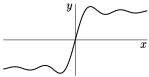
\includegraphics{graphE97_9}
\end{center}
\end{enumerate}
\end{Mquestion}

\begin{hint}
See Example \eref{CLP101}{eg:erf} in the
%\href{http://www.math.ubc.ca/%7Efeldman/m101/clp/clp_notes_101.pdf}{CLP--II text}.
CLP--II text.
For part (b), review  the fundamental theorem of calculus in \S \eref{CLP101}{sec fundamental}
of the
%\href{http://www.math.ubc.ca/%7Efeldman/m101/clp/clp_notes_101.pdf}{CLP--II text}.
CLP--II text.
For part (c), review  \S \eref{CLP101}{sec:AST} in the
%\href{http://www.math.ubc.ca/%7Efeldman/m101/clp/clp_notes_101.pdf}{CLP--II text}.
CLP--II text.

\end{hint}

\begin{answer}
(a)
$\displaystyle\Si(x)
=\sum\limits_{n=0}^\infty (-1)^n\ \frac{x^{2n+1}}{(2n+1)(2n+1)!}$
\qquad (b)
$x=\pi$
\qquad (c)
$1.8525$
\end{answer}

\begin{solution} (a)
Using the Taylor series expansion of $\sin x$ with $x=t$,
\begin{align*}
\sin t =\sum_{n=0}^\infty (-1)^n\frac{t^{2n+1}}{(2n+1)!}
&\implies \frac{\sin t}{t} =\sum_{n=0}^\infty (-1)^n\frac{t^{2n}}{(2n+1)!}
\end{align*}
So
\begin{align*}
\Si(x)
&=\int_0^x\frac{\sin t}{t}\,\dee{t}
=\sum_{n=0}^\infty (-1)^n\int_0^x \frac{t^{2n}}{(2n+1)!}\,\dee{t}
=\sum_{n=0}^\infty (-1)^n\ \frac{x^{2n+1}}{(2n+1)(2n+1)!}
\end{align*}

\noindent (b)
The critical points of $\Si(x)$ are the solutions of $\Si'(x)=0$.
By the fundamental theorem of calculus $\Si'(x)=\frac{\sin x}{x}$,
so the critical points of $\Si(x)$ are $x=\pm \pi, \pm 2\pi,\ \cdots$.
The absolute maximum occurs at $x=\pi$.

\noindent (c)
Substituting in $x=\pi$,
\begin{align*}
\Si(\pi)&=\sum_{n=0}^\infty (-1)^n\ \frac{\pi^{2n+1}}{(2n+1)(2n+1)!}\\
&=\pi-\frac{\pi^3}{3\cdot 3!}+\frac{\pi^5}{5\cdot 5!}-\frac{\pi^7}{7\cdot 7!}+\cdots\\
&=3.1416-1.7226+0.5100-0.0856+0.0091-0.0007+\cdots
\end{align*}
The series for $\Si(\pi)$ is an alternating series (that is, the sign alternates)
with successively smaller terms that converge to zero.
So the error introduced by truncating the series is no larger than the first omitted term. So
\begin{align*}
\Si(\pi)=3.1416-1.7226+0.5100-0.0856+0.0091=1.8525
\end{align*}
with an error of magnitude at most $0.0007+0.0005$ (the 0.0005 is the maximum
possible accumulated roundoff error in all five retained terms).

\end{solution}
%%%%%%%%%%%%%%%%%%%


\begin{Mquestion}[1997D]
  Let $\displaystyle I(x)=\int_0^x\frac{\cos t-1}{t^2}\,\dee{t}$.

\begin{enumerate}[(a)]
\item
Find the Maclaurin series for $I(x)$.
\item
Use this series to approximate $I(1)$ to within $\pm0.01$
\item
  Is your estimate in (b) greater than $I(1)$? Explain.
\end{enumerate}
\end{Mquestion}

\begin{hint}
See Example \eref{CLP101}{eg:erf} in the
%\href{http://www.math.ubc.ca/%7Efeldman/m101/clp/clp_notes_101.pdf}{CLP--II text}.
CLP--II text.
For parts (b) and (c), review  \S \eref{CLP101}{sec:AST} in the
%\href{http://www.math.ubc.ca/%7Efeldman/m101/clp/clp_notes_101.pdf}{CLP--II text}.
CLP--II text.

\end{hint}

\begin{answer}
(a)
$\displaystyle I(x)=\sum\limits_{n=1}^\infty(-1)^n\frac{x^{2n-1}}{(2n)!(2n-1)}$
\qquad (b)
$\displaystyle I(1)= -\frac{1}{2}+\frac{1}{4!3} \pm  \frac{1}{6!5}
        =-0.486\pm0.001$

\noindent (c)
$I(1)<-\dfrac{1}{2}+\dfrac{1}{4!3}$

\end{answer}

\begin{solution} (a)
Using the Taylor series expansion of $\cos t$,
\begin{alignat*}{3}
\cos t&=1-\frac{t^2}{2!}+\frac{t^4}{4!}-\frac{t^6}{6!}+\cdots
         &&=\sum_{n=0}^\infty(-1)^n\frac{t^{2n}}{(2n)!}\\
\frac{\cos t-1}{t^2}&= -\frac{1}{2!}+\frac{t^2}{4!}-\frac{t^4}{6!}+\cdots
         &&=\sum_{n=1}^\infty(-1)^n\frac{t^{2n-2}}{(2n)!}\\
I(x)=\int_0^x \frac{\cos t-1}{t^2}\,\dee{t}
      &=-\frac{x}{2!}+\frac{x^3}{4!3}-\frac{x^5}{6!5}+\cdots
      &&=\sum_{n=1}^\infty(-1)^n\frac{x^{2n-1}}{(2n)!(2n-1)}
\end{alignat*}


\noindent (b), (c)  Substituting in $x=1$,
\begin{align*}
I(1)&=-\frac{1}{2}+\frac{1}{4!3}-\frac{1}{6!5}
+\cdots\\
&=-0.5+0.0139-0.0003-\cdots\cr
&=-0.486\pm0.001
\end{align*}
The series for $I(1)$ is an alternating series with decreasing
successive terms that converge to zero. So approximating
$I(1)$ by $-\frac{1}{2}+\frac{1}{4!3}$ introduces an error
between $0$ and $-\frac{1}{6!5}$. Hence $I(1)<-\frac{1}{2}+\frac{1}{4!3}$.


\end{solution}
%%%%%%%%%%%%%%%%%%%


\begin{question}[1998A]
Let $\displaystyle I(x)=\int_0^x\frac{\cos t+t\sin t-1}{t^2}\,\dee{t}$

\begin{enumerate}[(a)]
\item
Find the Maclaurin series for $I(x)$.
\item
Use this series to approximate $I(1)$ to within $\pm0.001$
\item
Is your estimate in (b) greater than or less than $I(1)$?
\end{enumerate}
\end{question}

\begin{hint}
See Example \eref{CLP101}{eg:erf} in the
%\href{http://www.math.ubc.ca/%7Efeldman/m101/clp/clp_notes_101.pdf}{CLP--II text}.
CLP--II text.
For parts (b) and (c), review  \S \eref{CLP101}{sec:AST} in the
%\href{http://www.math.ubc.ca/%7Efeldman/m101/clp/clp_notes_101.pdf}{CLP--II text}.
CLP--II text.

\end{hint}

\begin{answer}
(a)
 $\displaystyle I(x)=\sum_{n=1}^\infty (-1)^{n+1}\frac{x^{2n-1}}{(2n)!}= \frac{1}{2!}x-\frac{1}{4!}x^3+\frac{1}{6!}x^5-\frac{1}{8!}x^8+\cdots$
\\ (b)
 0.460
\qquad (c)
 $\displaystyle I(1)<\frac{1}{2!}-\frac{1}{4!}+\frac{1}{6!}<0.460$

\end{answer}

\begin{solution} (a)
Using the Taylor series expansions of $\sin x$ and $\cos x$ with $x=t$,
\begingroup
\allowdisplaybreaks
\begin{align*}
\sin t &= \sum_{n=0}^\infty (-1)^n\frac{t^{2n+1}}{(2n+1)!}&=& t-\frac{t^3}{3!}+\frac{t^5}{5!}-\frac{t^7}{7!}+\cdots\\
\color{red}t\sin t &= \sum_{n=0}^\infty (-1)^n\frac{t^{2n+2}}{(2n+1)!}&=&\color{red}\phantom{1-\ }t^2-\frac{t^4}{3!}+\frac{t^6}{5!}-\frac{t^8}{7!}+\cdots\\
&=\color{red} -\sum_{n=1}^\infty (-1)^n\frac{t^{2n}}{(2n-1)!}\\
\cos t &=\sum_{n=0}^\infty (-1)^n\frac{t^{2n}}{(2n)!}&=& 1-\frac{t^2}{2!}+\frac{t^4}{4!}-\frac{t^6}{6!}+\frac{t^8}{8!}+\cdots\\
\color{blue}\cos t-1 &=\color{blue}\sum_{n=1}^\infty (-1)^n\frac{t^{2n}}{(2n)!}&=&\color{blue} -\frac{t^2}{2!}+\frac{t^4}{4!}-\frac{t^6}{6!}+\frac{t^8}{8!}+\cdots\\
\textcolor{blue}{\cos t} + \textcolor{red}{t\sin t}\textcolor{blue}{ -1}&=\color{blue}\sum_{n=1}^\infty (-1)^n\frac{t^{2n}}{(2n)!}\color{red}-\sum_{n=1}^\infty (-1)^n\frac{t^{2n}}{(2n-1)!}
\\&=\sum_{n=1}^\infty (-1)^nt^{2n}\left(\frac{1}{(2n)!}-\frac{1}{(2n-1)!}\right)&=&\Big(1-\frac{1}{2!}\Big)t^2
-\Big(\frac{1}{3!}-\frac{1}{4!}\Big)t^4
+\cdots\\
&=\sum_{n=1}^\infty (-1)^nt^{2n}\left(\frac{1}{(2n)!}-\frac{2n}{(2n)!}\right)\\
&=\sum_{n=1}^\infty (-1)^nt^{2n}\left(\frac{1-2n}{(2n)!}\right)
&=&\Big(\frac{2}{2!}-\frac{1}{2!}\Big)t^2
-\Big(\frac{4}{4!}-\frac{1}{4!}\Big)t^4
+\cdots\\
&=\sum_{n=1}^\infty (-1)^{n+1}t^{2n}\left(\frac{2n-1}{(2n)!}\right)
&=&\frac{1}{2!}t^2-\frac{3}{4!}t^4
+\frac{5}{6!}t^6
-\frac{7}{8!}t^8+\cdots\\
\frac{\cos t + t\sin t -1}{t^2}&=\sum_{n=1}^\infty (-1)^{n+1}t^{2n-2}\left(\frac{2n-1}{(2n)!}\right)
&=&\frac{1}{2!}t-\frac{3}{4!}t^2
+\frac{5}{6!}t^4
-\frac{7}{8!}t^6+\cdots\\
\end{align*}
\endgroup
Now, we're ready to integrate.
\begin{align*}
I(x)=\int_0^x\left( \frac{\cos t + t\sin t -1}{t^2}\right)&=\int_0^x \left(\sum_{n=1}^\infty (-1)^{n+1}t^{2n-2}\left(\frac{2n-1}{(2n)!} \right)\right) \dee{t}\\
&= \left[\sum_{n=1}^\infty (-1)^{n+1}\frac{t^{2n-1}}{(2n)!}\right]_0^x\\
&=\sum_{n=1}^\infty (-1)^{n+1}\frac{x^{2n-1}}{(2n)!}
\end{align*}

\noindent (b)
$I(1)=\frac{1}{2!}-\frac{1}{4!}+\frac{1}{6!}-\frac{1}{8!}+\cdots
=0.5-0.041\dot6+0.00139-0.000024+\cdots=\boxed{0.460}\,$.
The error analysis is in part (c).

\noindent (c) The series for $I(1)$ is an alternating series with decreasing
successive terms that convege to zero. So approximating
$I(1)$ by $\frac{1}{2!}-\frac{1}{4!}+\frac{1}{6!}$ introduces an error
between $0$ and $-\frac{1}{8!}$. So  $I(1)<\frac{1}{2!}-\frac{1}{4!}+\frac{1}{6!}<0.460$.

\end{solution}
%%%%%%%%%%%%%%%%%%%

\begin{question}[2016A]
Define
$
{\displaystyle f(x) = \int_0^x\frac{1-e^{-t}}{t}\ \dee{t}}
$.
\begin{enumerate}[(a)]
\item
Show that the Maclaurin series for $f(x)$ is
$\displaystyle\sum_{n=1}^\infty \frac{(-1)^{n-1}}{n\cdot n!} x^n$.

\item
Use the ratio test to determine the values of $x$ for which
the Maclaurin series
$\displaystyle\sum_{n=1}^\infty \frac{(-1)^{n-1}}{n\cdot n!} x^n$ converges.
\end{enumerate}
\end{question}

%\begin{hint}
%\end{hint}

\begin{answer}
(a) See the solution.
\qquad
(b) The series converges for all $x$.
\end{answer}

\begin{solution} (a)
Substituting $x=-t$ into the known power series
$e^x = 1 + x +\frac{x^2}{2!}+\frac{x^3}{3!} + \frac{x^4}{4!} + \cdots$,
we see that:
\begin{align*}
e^{-t}&= 1  - t +\frac{t^2}{2!}-\frac{t^3}{3!} + \frac{t^4}{4!} - \cdots \\
1-e^{-t}&=  t - \frac{t^2}{2!}+ \frac{t^3}{3!} - \frac{t^4}{4!} + \cdots \\
\frac{1-e^{-t}}{t}&=  1 - \frac{t}{2!}+ \frac{t^2}{3!} - \frac{t^3}{4!} + \cdots \\
\int \frac{1-e^{-t}}{t}\ \dee{t}&=  C + x - \frac{x^2}{2\cdot 2!}
                   + \frac{x^3}{3\cdot 3!} - \frac{x^4}{4\cdot 4!} + \cdots
\end{align*}
Finally, $f(0) = 0$ (since $f(0)$ is an integral from $0$ to $0$) and so $C=0$. Therefore
\begin{align*}
f(x) = \int_0^x\frac{1-e^{-t}}{t}\ \dee{t} =  x - \frac{x^2}{2\cdot 2!} + \frac{x^3}{3\cdot 3!} - \frac{x^4}{4\cdot 4!} + \cdots.
\end{align*}

\medskip\noindent
We can also do this calculation entirely in summation notation:
$e^{x}= \displaystyle\sum\limits_{n=0}^\infty \frac{x^n}{n!}$, and so
\begin{align*}
e^{-t}&= \sum_{n=0}^\infty \frac{(-t)^n}{n!}
  =1+ \sum_{n=1}^\infty \frac{(-1)^nt^n}{n!} \\
1-e^{-t}&= - \sum_{n=1}^\infty \frac{(-1)^nt^n}{n!} = \sum_{n=1}^\infty \frac{(-1)^{n-1} t^n}{n!} \\
\frac{1-e^{-t}}{t}&= \sum_{n=1}^\infty \frac{(-1)^{n-1} t^{n-1}}{n!} \\
\hskip-90pt f(x) = \int_0^x\frac{1-e^{-t}}{t}\ \dee{t}
&= \sum_{n=1}^\infty \frac{(-1)^{n-1} x^n}{n\cdot n!}
\end{align*}

\noindent (b)
We set $a_n=A_nx^n = \dfrac{(-1)^{n-1}}{n\cdot n!} x^n$ and apply
the ratio test.
\begin{align*}
\lim_{n\rightarrow\infty}\Big|\frac{a_{n+1}}{a_n}\Big|
&=\lim_{n\rightarrow\infty}
   \bigg|\frac{{(-1)^{n}}x^{n+1}/{((n+1)\cdot (n+1)!)}}
                {{(-1)^{n-1}}x^n/{(n\cdot n!)}}\bigg| \\
&=\lim_{n\rightarrow\infty}
   \bigg( \frac{|x|^{n+1}}{|x|^n} \frac{n\cdot n!}{(n+1)\cdot (n+1)!} \bigg) \\
&=\lim_{n\rightarrow\infty}
      \bigg( |x|\frac{n}{(n+1)^2} \bigg)
\qquad\text{since $(n+1)!=(n+1)\,n!$}
\\
&=0
\end{align*}
This is smaller than $1$ no matter what $x$ is.
So the series converges for all $x$.


\end{solution}
%%%%%%%%%%%%%%%%%%%%%%%%%%%%%%%%


\begin{question}[1998A]
 Show that $\displaystyle \int_0^1\frac{x^3}{e^x-1}\,\dee{x}\le\frac{1}{3}$.
\end{question}

\begin{hint}
Use the Maclaurin series for $e^x$.
\end{hint}

\begin{answer}
See the solution.
\end{answer}

\begin{solution}
\begin{align*}
&e^x=1+x+\frac{x^2}{2!}+\frac{x^3}{3!}+\cdots
\ge 1+x\qquad\hbox{for all $x\ge 0$}\\
&\implies   e^x-1\ge x \\
&\implies   \frac{x^3}{e^x-1}\le \frac{x^3}{x} = x^2 \\
&\implies   \int_0^1\frac{x^3}{e^x-1}\,\dee{x} \le \int_0^1 x^2\,\dee{x}=\frac{1}{3}
\end{align*}


\end{solution}
%%%%%%%%%%%%%%%%%%%



\begin{question}[M121 2012A]
Let $\displaystyle \cosh(x) =\frac{e^x+e^{-x}}{2}$.
\begin{enumerate}[(a)]
\item
Find the power series expansion of $\cosh(x)$ about $x_0 = 0$ and
determine its interval of convergence.
\item
Show that $3\frac{2}{3}\le \cosh(2) \le 3\frac{2}{3} + 0.1$.
\item
Show that $\cosh(t) \le e^{\frac{1}{2}t^2}$ for all $t$.
\end{enumerate}
\end{question}

\begin{hint}
For part (c), compare two power series term-by-term.
\end{hint}

\begin{answer}
(a)
$\cosh(x)=\displaystyle \sum\limits_{\genfrac{}{}{0pt}{}{n=0}{n\text{ even}}}^\infty
                                      \frac{x^n}{n!}
         = \sum\limits_{n=0}^\infty\frac{x^{2n}}{(2n)!}$ for all $x$.
\end{answer}

\begin{solution} (a) We know that
$e^x = \sum\limits_{n=0}^\infty \frac{x^n}{n!}$ for all $x$.
Replacing $x$ by $-x$, we also have
$e^{-x} = \sum\limits_{n=0}^\infty \frac{(-x)^n}{n!}$ for all $x$
and hence
\begin{align*}
\cosh(x) =\frac{1}{2}\big[e^x+e^{-x}\big]
         =\frac{1}{2}\Big[\sum_{n=0}^\infty \frac{x^n}{n!}
                         + \sum_{n=0}^\infty \frac{(-x)^n}{n!}\Big]
         = \sum_{\genfrac{}{}{0pt}{}{n=0}{n\text{ even}}}^\infty\frac{x^n}{n!}
         = \sum_{n=0}^\infty\frac{x^{2n}}{(2n)!}
\end{align*}
for all $x$. In particular, the interval of convergence is all real numbers.

\noindent (b) Using the power series expansion of part (a),
\begin{align*}
\cosh(2) &= 1 +\frac{2^2}{2!}+\frac{2^4}{4!}
                    +\sum_{n=3}^\infty\frac{2^{2n}}{(2n)!}
         = 3\frac{2}{3}
                    +\sum_{n=3}^\infty\frac{2^{2n}}{(2n)!}
\end{align*}
So it suffices to show that $\sum_{n=3}^\infty\frac{2^{2n}}{(2n)!}\le 0.1$.
Let's write $b_n = \frac{2^{2n}}{(2n)!}$. The first term in
$\sum_{n=3}^\infty\frac{2^{2n}}{(2n)!}$ is
\begin{equation*}
b_3 = \frac{2^6}{6!}
    = \frac{2^6}{6 \times 5 \times 4 \times 3\times 2}
    = \frac{4}{45}
\end{equation*}
The ratio between successive terms in $\sum_{n=3}^\infty\frac{2^{2n}}{(2n)!}$
is
\begin{align*}
\frac{b_{n+1}}{b_n}
= \frac{2^{2n+2}/2^{2n}}{(2n+2)!/(2n)!}
=\frac{4}{(2n+2)(2n+1)}
\le \frac{4}{8\times 7}
=\frac{1}{14}\qquad
\text{for all }n\ge 3
\end{align*}
Hence
\begin{align*}
\sum_{n=3}^\infty\frac{2^{2n}}{(2n)!}
&\le \overbrace{\frac{4}{45}}^{b_3}
    + \overbrace{\frac{4}{45}\times \frac{1}{14}}^{b_4\le}
    + \overbrace{\frac{4}{45}\times \frac{1}{14^2}}^{b_5\le}
    + \overbrace{\frac{4}{45}\times \frac{1}{14^3}}^{b_6\le}
    + \cdots\\
&=\frac{4}{45}\,\frac{1}{1-\frac{1}{14}}
=\frac{4}{45}\,\frac{14}{13}
=\frac{56}{585}<\frac{1}{10}
\end{align*}


\noindent (c) Comparing
\begin{equation*}
\cosh(t) = \sum_{n=0}^\infty\frac{t^{2n}}{(2n)!}
 = \sum_{n=0}^\infty\frac{{(t^2)}^n}{(2n)!}
\qquad\text{and}\qquad
e^{\frac{1}{2}t^2}
    = \sum_{n=0}^\infty\frac{{(\frac{1}{2}t^2)}^n}{n!}
    = \sum_{n=0}^\infty\frac{{(t^2)}^n}{2^n n!}
\end{equation*}
we see that it suffices to show that $(2n)! \ge 2^n n!$.
Now. for all $n\ge 1$,
\begin{align*}
(2n)! &=\overbrace{1\times 2\times\cdots\times n}^{n\text{ factors}}
      \overbrace{(n+1)\times (n+2)\times\cdots\times 2n}^{n\text{ factors}} \\
&\ge\overbrace{1\times 2\times\cdots\times n}^{n\text{ factors}}
      \overbrace{2\times 2\times\cdots\times 2}^{n\text{ factors}} \\
&=2^n\, n!
\end{align*}

\end{solution}












%%%%%%%%%%%%%%%%%%%


\begin{Mquestion}
The law of the instrument says ``If you have a hammer then everything looks like a nail'' --- it is really a
description of the ``tendency of jobs to be adapted to tools rather than adapting tools to jobs.''\footnote{Quote
from Silvan Tomkins's \emph{Computer Simulation of Personality: Frontier of Psychological Theory}. See also
Birmingham screwdrivers.} Anyway, this is a long way of saying that just because we know how to compute things
using Taylor series doesn't mean we should neglect other techniques.
	\begin{enumerate}[(a)]
		\item Using Newton's method, approximate the constant $\sqrt[3]{2}$ as a root of the function $g(x)=x^3-2$. Using a calculator, make your estimation accurate to within 0.01.
		\item You may assume without proof that
		\[\sqrt[3]{x}=1+\frac{1}{6}(x-1)+\sum_{n=2}^\infty(-1)^{n-1}\frac{(2)(5)(8)\cdots(3n-4)}{3^n\, n!}(x-1)^n.\]
		for all real numbers $x$. Using the fact that this is an alternating series, how many terms would you have to add for the partial sum to estimate $\sqrt[3]{2}$ with an error less than 0.01?
	\end{enumerate}


\end{Mquestion}
\begin{hint}
For Newton's method, recall we approximate a root of the function $g(x)$ in iterations: given an approximation $x_n$, our next approximation is $x_{n+1}=x_n-\dfrac{g(x_n)}{g'(x_n)}$.

To gauge your error, note that from approximation to approximation, the first digits stabilize. Keep refining your approximation until the first two digits stop changing.
\end{hint}
\begin{answer}
(a) $\sqrt[3]{3}\approx 1.26$\qquad (b) 12 terms ($S_{11}$)
\end{answer}
\begin{solution}

	\begin{enumerate}[(a)]
		\item
		For Newton's method, recall we approximate a root of the function $g(x)$ in iterations: given an approximation $x_n$, our next approximation is $x_{n+1}=x_n-\dfrac{g(x_n)}{g'(x_n)}$. In our case,
\[x_{n+1}=x_n - \frac{x_n^3-2}{3x_n^2}=\frac23\left(x_n+\frac{1}{x_n^2}\right).\]

We want to start somewhere reasonably close to the actual root we want, so let's set $x_0=1$. (Your starting point may vary.)

\begin{align*}
x_0&=1 &&\implies x_1=\dfrac23\left(1+\frac11\right)=\dfrac{4}{3}&\approx&1.3333\\
 x_1&=\dfrac43 &&\implies x_2=\dfrac23\left(\frac43+\frac{9}{16}\right)=\dfrac{91}{72}&\approx&1.2639\\
  x_2&=\dfrac{91}{72} &&\implies x_3=\dfrac23\left(\dfrac{91}{72}+\dfrac{72^2}{91^2}\right)=\dfrac{1126819 }{894348 }&\approx&1.2599\\
    x_3&=\dfrac{1126819 }{894348 } &&\implies x_4=\dfrac23\left(\dfrac{1126819 }{894348 }+\dfrac{894348^2}{1126819^2}\right)&\approx&1.2599
\end{align*}
So, $\sqrt[3]{2}\approx 1.26$.
		\item
		We'll evaluate the given series at $x=2$. This yields the series
		\[\sqrt[3]{2}=1+\frac{1}{6}+\sum_{n=2}^\infty(-1)^{n-1}\frac{(2)(5)(8)\cdots(3n-4)}{3^n\, n!}.\]
		This series is alternating, so if we use the partial sum $S_N$, our absolute error is at most \[|a_{N+1}|=\frac{(2)(5)(8)\cdots(3N-1)}{3^{N+1}\, (N+1)!}\]
		(if $N \ge 2$). We want to know which value of $N$ makes this at most 0.01. We test several values.

\begin{center}
\begin{tabular}{| m{1cm} | m{10cm} |}
\hline
$N$&$|a_{N+1}|$\\[1em]
\hline
3& $\dfrac{(2)(5)(8)}{3^4\cdot 4!}\approx 0.04$\\[1em]
\hline
4 & $\dfrac{(2)(5)(8)(11)}{3^5\, 5!}\approx 0.03$\\[1em]
\hline
5 & $\dfrac{(2)(5)(8)(11)(14)}{3^6\, 6!}\approx 0.023$\\[1em]
\hline
6 & $\dfrac{(2)(5)(8)(11)(14)(17)}{3^7\, 7!}\approx 0.019$\\[1em]
\hline
7 & $\dfrac{(2)(5)(8)(11)(14)(17)(20)}{3^8\, 8!}\approx 0.016$\\[1em]
\hline
8 & $\dfrac{(2)(5)(8)(11)(14)(17)(20)(23)}{3^9\, 9!}\approx 0.013$\\[1em]
\hline
9 & $\dfrac{(2)(5)(8)(11)(14)(17)(20)(23)(26)}{3^{10}\, 10!}\approx 0.012$\\[1em]
\hline
10 & $\dfrac{(2)(5)(8)(11)(14)(17)(20)(23)(26)(29)}{3^{11}\, 11!}\approx 0.0103$\\[1em]
\hline
11 & $\dfrac{(2)(5)(8)(11)(14)(17)(20)(23)(26)(29)(32)}{3^{12}\, 12!}\approx 0.009$\\[1em]
\hline
\end{tabular}
\end{center}
So, the approximation $S_{11}$ has a sufficiently small error. That is, we would add up the first twelve terms.
	\end{enumerate}
\end{solution}
%%%%%%%%%%%%%%%%%%%

%%%%%%%%%%%%%%%%%%%
\begin{question}
Let $f(x)=\arctan(x^3)$. Write $f^{(10)}\left(\frac{1}{5} \right)$ as a sum of rational numbers with an error less than $10^{-6}$ using the Maclaurin series for arctangent.
\end{question}
\begin{hint}
First, modify your known Maclaurin series for arctangent into a Maclaurin series for $f(x)$. This series is not hard to repeatedly differentiate, so use it to find a power series for $f^{(10)}(x)$.
\end{hint}
\begin{answer}
$\displaystyle \frac{15!}{5!\cdot5^6}-\frac{21!}{7!\cdot 11!\cdot 5^{11}}+\frac{27!}{9!\cdot 17!\cdot 5^{17}}-\frac{33!}{11!\cdot 23!\cdot 5^{23}}$
\end{answer}
\begin{solution}

	Our plan is as follows:
	\begin{itemize}
	\item Make a Taylor series for $f(x)$
	\item Calculate the tenth derivative of the Taylor series of $f(x)$.
	\item Decide how many terms we need to add to achieve the desired accuracy.
	\item Approximate $f^{(10)}\left(\frac15\right)$ with a partial sum.
	\end{itemize}

We know that the Taylor series for $\arctan x$ is $\displaystyle\sum_{n=0}^\infty (-1)^n\frac{x^{2n+1}}{2n+1}$, which converges for $-1\le x\le1$. So, the Taylor series for $\arctan(x^3)$ is
\[f(x)=\arctan(x^3)=\sum_{n=0}^\infty (-1)^n\frac{(x^3)^{2n+1}}{2n+1}
=\sum_{n=0}^\infty (-1)^n\frac{x^{6n+3}}{2n+1}\]
It is much easier to differentiate this series many times than it is to differentiate $\arctan(x^3)$ directly many times.
\begin{align*}
f'(x)&=\sum_{n=0}^\infty (-1)^n\frac{(6n+3)x^{6n+2}}{2n+1}\\
f''(x)&=\sum_{n=0}^\infty (-1)^n\frac{(6n+3)(6n+2)x^{6n+1}}{2n+1}\\
f'''(x)&=\sum_{n=0}^\infty (-1)^n\frac{(6n+3)(6n+2)(6n+1)x^{6n}}{2n+1}\\
\vdots&\\
f^{(10)}(x)&=\sum_{n=0}^\infty (-1)^n\frac{(6n+3)(6n+2)(6n+1)\cdots(6n-6)x^{6n-7}}{2n+1}\\
&=\sum_{n=2}^\infty (-1)^n\frac{(6n+3)(6n+2)(6n+1)\cdots(6n-6)x^{6n-7}}{2n+1}\\
&=\sum_{n=2}^\infty (-1)^n\frac{(6n+3)!}{(2n+1)(6n-7)!}x^{6n-7}\\
f^{(10)}\left(\frac{1}{5}\right)&=\sum_{n=2}^\infty (-1)^n\frac{(6n+3)!}{(2n+1)(6n-7)!\cdot 5^{6n-7}}
\end{align*}
(Notice, after ten differentiations, the terms $a_0$ and $a_1$ are both zero.)

Since this is an alternating series, the absolute error involved in using the approximation $S_N$ is at most
\[|a_{N+1}|=\frac{(6N+9)!}{(2N+3)(6N-1)!\cdot 5^{6N-1}}\]
By testing a few values of $N$, we find
\[|a_6|=|a_{5+1}|=\frac{39!}{(13)(29!)\cdot 5^{29}}\approx 0.00000095<10^{-6}\]
So, $S_5$ is a sufficient approximation. That is,
\begin{align*}
f^{(10)}\left(\frac15\right)&\approx \sum_{n=2}^5 (-1)^n\frac{(6n+3)!}{(2n+1)(6n-7)!\cdot 5^{6n-7}}\\
&=(-1)^2\frac{15!}{5\cdot 5!\cdot 5^{5}}+(-1)^3\frac{21!}{7!\cdot 11!\cdot 5^{11}}+
(-1)^4\frac{27!}{9!\cdot 17!\cdot 5^{17}}+
(-1)^5\frac{33!}{11!\cdot 23!\cdot 5^{23}}\\
&=\frac{15!}{5!\cdot5^6}-\frac{21!}{7!\cdot 11!\cdot 5^{11}}+\frac{27!}{9!\cdot 17!\cdot 5^{17}}-\frac{33!}{11!\cdot 23!\cdot 5^{23}}
\end{align*}
Remark: if we had calculated $f^{(10)}(1/5)$ directly, using derivative rules instead of series, we would have found an exact value; however, our value here is easier to find, and is highly accurate (if not exact).
\end{solution}
%%%%%%%%%%%%%%%%%%%

%%%%%%%%%%%%%%%%%%%

%%%%%%%%%%%%%%%%%%%
\begin{question}
Consider the following function:
\[f(x)=\begin{cases}
e^{-1/x^2} & x \neq 0\\
0 & x=0
\end{cases}\]
\begin{enumerate}[(a)]
	\item Sketch $y=f(x)$.
	\item Assume (without proof) that $f^{(n)}(0)=0$ for all whole numbers $n$. Find the Maclaurin series for $f(x)$.
	\item Where does the Maclaurin series for $f(x)$ converge?
	\item For which values of $x$ is $f(x)$ equal to its Maclaurin series?
	\end{enumerate}
\end{question}
\begin{hint}
	Remember $e^x$ is never negative for any real number $x$.
\end{hint}
\begin{answer}
	(a) 	\begin{tikzpicture}
	\YEaaxis{4}{4}{.5}{2.5}
	\draw (0,0) node[vertex]{};
	\YEycoord{2}{1}
	\YExcoord{-1.63}{-\sqrt{2/3}}
	\YExcoord{1.63}{\sqrt{2/3}}
	\draw[thick] plot[domain=-2:-.05, scale=2](\x,{exp(-1/(\x*\x))});
	\draw[thick] plot[domain=-.05:2, scale=2](\x,{exp(-1/(\x*\x))});
	\draw (4,2) node[right]{$y=f(x)$};
	\end{tikzpicture}

	(b) the constant function 0 \qquad (c) everywhere \qquad (d) only at $x=0$
\end{answer}
\begin{solution}
\begin{enumerate}[(a)]
	\item
	To sketch $y=f(x)$, we note the following:
	\begin{itemize}
	\item $f(x)$ is never negative.
	\item $\lim\limits_{x \to \pm \infty} f(x)=e^0=1$, so the curve has horizontal asymptotes in both directions at $y=1$.
	\item $\lim\limits_{x \to \pm 0} f(x)=\lim\limits_{x \to \pm 0} \frac{1}{e^{1/x^2}}=\lim\limits_{u \to +\infty}\frac{1}{e^u}=0=f(0)$, so the curve is continuous at $x=0$.
	\item For $x\neq 0$, $f'(x)=\frac{2}{x^3}e^{-1/x^2}$, so our curve is decreasing on $(-\infty,0)$ and increasing on $(0,\infty)$
	\item For $x\neq 0$,  $f''(x)=2x^{-6}(2-3x^2)e^{-1/x^2}$, so our curve is concave up on $(-\sqrt{2/3},\sqrt{2/3})$, and concave down elsewhere.
\end{itemize}
	\begin{center}
		\begin{tikzpicture}
		\YEaaxis{4}{4}{.5}{2.5}
		\draw (0,0) node[vertex]{};
		\YEycoord{2}{1}
		\YExcoord{-1.63}{-\sqrt{2/3}}
		\YExcoord{1.63}{\sqrt{2/3}}
		\draw[thick] plot[domain=-2:-.05, scale=2](\x,{exp(-1/(\x*\x))});
		\draw[thick] plot[domain=-.05:2, scale=2](\x,{exp(-1/(\x*\x))});
		\draw (4,2) node[right]{$y=f(x)$};
		\end{tikzpicture}
		\end{center}
\item Since $f^{(n)}(0)=0$ for all whole $n$ (that is, the graph is really quite flat at the origin), and since $f(0)=0$, the Maclaurin series for $f(x)$ is $\displaystyle\sum_{n=0}^\infty \frac{0}{n!}x^n=0$.
\item The Maclaurin series converges for all real values of $x$ (to the constant 0).
\item Since $e^y>0$ for any real $y$, we see $f(x)=0$ only when $x=0$. So, $f(x)$ is only equal to its Maclaurin series at the single point $x=0$.
	\end{enumerate}
Remark: the function $f(x)$ is an example of a function whose Maclaurin series converges, but not to $f(x)$! To describe this behaviour, we say $f(x)$ is \emph{non-analytic}.
\end{solution}

%%%%%%%%%%%%%%%%%%%
\begin{Mquestion}
Suppose $f(x)$ is an odd function, and $f(x)=\displaystyle\sum_{n=0}^\infty\frac{f^{(n)}(0)}{n!}x^n$. Simplify
$\displaystyle\sum_{n=0}^\infty \dfrac{f^{(2n)}(0)}{(2n)!}x^{2n}$.
\end{Mquestion}
\begin{hint}
Since $f(x)$ is odd, $f(-x)=-f(x)$ for all $x$ in its domain. Consider the even-indexed terms and odd-indexed terms of the Taylor series.
\end{hint}
\begin{answer}
	$0$
\end{answer}
\begin{solution}
	\begin{description}
\item[Solution 1:]
		Since $f(x)$ is odd, $f(-x)=-f(x)$ for all $x$ in its domain. We plug this into our power series, then consider the even-indexed terms and the odd-indexed terms separately.
\begin{align*}
f(-x)&=-f(x)\\
\sum_{n=0}^\infty\frac{f^{(n)}(0)}{n!}(-x)^n&=-\sum_{n=0}^\infty\frac{f^{(n)}(0)}{n!}x^n\\
\textcolor{red}{\sum_{n=0}^\infty\frac{f^{(2n+1)}(0)}{(2n+1)!}(-x)^{2n+1}}+
\textcolor{blue}{\sum_{n=0}^\infty\frac{f^{(2n)}(0)}{(2n)!}(-x)^{2n}}&=\textcolor{red}{-\sum_{n=0}^\infty\frac{f^{(2n+1)}(0)}{n!}x^{2n+1}}\textcolor{blue}{-\sum_{n=0}^\infty\frac{f^{(2n)}(0)}{n!}x^{2n}}\\
\textcolor{red}{-\sum_{n=0}^\infty\frac{f^{(2n+1)}(0)}{(2n+1)!}x^{2n+1}}+
\textcolor{blue}{\sum_{n=0}^\infty\frac{f^{(2n)}(0)}{(2n)!}x^{2n}}&=\textcolor{red}{-\sum_{n=0}^\infty\frac{f^{(2n+1)}(0)}{n!}x^{2n+1}}\textcolor{blue}{-\sum_{n=0}^\infty\frac{f^{(2n)}(0)}{n!}x^{2n}}\\
\textcolor{blue}{\sum_{n=0}^\infty\frac{f^{(2n)}(0)}{(2n)!}x^{2n}}&=\textcolor{blue}{-\sum_{n=0}^\infty\frac{f^{(2n)}(0)}{n!}x^{2n}}\\
2\textcolor{blue}{\sum_{n=0}^\infty\frac{f^{(2n)}(0)}{(2n)!}x^{2n}}&=0\\
\textcolor{blue}{\sum_{n=0}^\infty\frac{f^{(2n)}(0)}{(2n)!}x^{2n}}&=0
\end{align*}

\item[Solution 2:]	Alternately, we could note the following:
	\begin{itemize}
	\item Since all derivative of $f(x)$ exist, all its derivatives are continuous.
		\item The derivative of an odd function is even, and the derivative of an even function is odd.
		\item So, the even-indexed derivatives of $f(x)$ are continuous, odd functions.
		\item Every continuous, odd function passes through the origin. That is, $f^{(2n)}(0)=0$.
		\item So, every term in the series is $0$.
		\end{itemize}
	\end{description}
\end{solution}
%%%%%%%%%%%%%%%%%%%
